\documentclass[12pt]{article}
\usepackage[margin=1in]{geometry}
\usepackage{textcomp}
\usepackage{gensymb}
\usepackage{graphicx}
\usepackage{epstopdf}
\usepackage{textgreek}
\usepackage{titlesec}
\usepackage{float}
\usepackage{cite}
%\usepackage{natbib}
\usepackage[articletitle=true,doi=true]{achemso}

\titlespacing*{\section} {0pt}{0mm}{0mm}
\titlespacing*{\subsection} {0pt}{0mm}{0mm}

\let\bf\textbf

\begin{document}
\linespread{1.25}
\raggedright
\setlength{\parskip}{6pt}

\section*{(Chalcone Project)}

David Behrle

\subsection*{INTRODUCTION}
Malaria remains a major public health issue with nearly 230 million cases estimated worldwide in 2019, the vast majority of which were reported in Africa owing to infection by protozoan parasites in the genus $Plasmodium$, most notably $Plasmodium\; falciparum$.\cite{Fikadu2023} Historically, chloroquine and its derivatives have been used to treat malaria however, the emergence of chloroquine-resistant strains of $P.\; falciparum$ has greatly decreased the efficacy of these treatments creating an urgent need for alternative antimalarial compounds.\cite{Fikadu2023,Yadav2012} Chalcones are a class of \textalpha,\textbeta-unsaturated ketones belonging to the flavonoid family which remain of significant interest due to their relatively simple synthetic chemistry and diverse application as scaffolds in medicinal chemistry.\cite{Qin2020} Discovery of the antimalarial activity of the naturally occuring chalcone Licochalcone A, originally isolated from Chinese licorice roots, has prompted research into chalcones and chalcone hybrids as antimalarial candidates.\cite{Cheng2020,Chen1994} Hybridization has been explored as a method for overcoming drug resistance in $P.\; falciparum$, this is supported by the observation that many chloroquine derivatives and analogs retain activity against chloroquine-resistant strains of $P.\; falciparum$.\cite{Cheng2020,Sashidhara2012} Chloroquine-chalcone based hybrids have been shown to have potent antimalarial activity against chloroquine-resistant $P.\; falciparum$ in vitro when compared with chloroquine.\cite{Sashidhara2012} Likewise, triazole linked chalcones, ferrocenyl chalcones, and caffeine based chalcones among others have been evaluated as potential antimalarial, antitrypanosomal, antileishmanial, and antiplasmodial agents.\cite{Qin2020,Singh2017,Insuasty2015} Structure-activity relationship studies of various chalcone derivatives have shown that different structural requirements exist for antimalarial and antileishmanial activity respectively, with the A ring being more significant in antileishmanial activity compared with antimalarial activity in which both A and B rings are important.\cite{Liu2003} Stereoisomerism has also been shown to have an effect on the antimalarial activity of chalcone derivatives. Synthesis and evaluation of conformationally restricted derivatives of known antiplasmodial chalcones has demonstrated that Z-locked chalcone derivatives are effectively inactive while E-locked analogs show equivalent activity and potency to the parent chalcone.\cite{Larsen2005} Chalcone derivatives lacking the \textalpha,\textbeta-unsaturated ketone bridge exhibit significantly less antimalarial activity, with saturated analogs showing a 10-fold decrease in antimalarial activity.\cite{Li1995}
\subsection*{METHODS AND RESULTS}
\bf{Instrumentation.} Nuclear magnetic resonance (NMR) spectra were recorded on a Bruker Ultrashield™ (CDCl$_3$, 400 MHz) calibrated using deuterated solvent (CDCl$_3$: $^1$H NMR: 7.26 ppm). IR spectra were recorded on a Nicolet Summit™ FTIR spectrometer. UV-Vis spectra were recorded on a Vernier Fluorescence/UV-Vis spectrophotometer.

\begin{figure}[H]
    \centering
    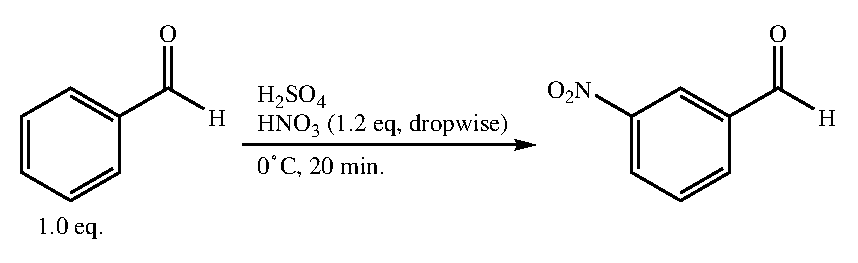
\includegraphics[scale=0.8]{schemes/nitration.eps}
    \caption{Nitration of benzaldehyde}
\end{figure}
\bf{Procedure.} Benzaldehyde (10.4 g, 98.0 mmol) was added to a 250 mL round bottom flask and cooled to 0°C, followed by addition of sulfuric acid (30 mL). To this solution, nitric acid (7 mL) was added dropwise over 10 minutes, and allowed to stir for 10 minutes. Reaction progress was monitored with TLC (9:1 hexanes:EtOAc). When the reaction was complete, the reaction mixture was quenched with ice (\textasciitilde 50 mL), the crude product was filtered by vacuum, and recrystallized from isopropanol.

\noindent\bf{3-nitrobenzaldehyde:} yellow crystals. Hexanes:EtOAc 9:1 R\textsubscript{f} = 0.43. \bf{$^1$H-NMR} (400 MHz, CDCl$_3$): \textdelta\hspace{0mm} 7.761 - 7.801 (t, 1H), 8.236 - 8.256 (d, 1H), 8.487 - 8.516 (dq, 1H), 8.728 (s, 1H), 10.134 (s, 1H). \bf{IR} (neat): 3069, 2981, 2884, 1698, 1523, 1348, 1198 cm$^{-1}$ \bf{UV-Vis:} \textlambda\textsubscript{max} = 220 nm. \bf{MP:} 47.6\degree C. \bf{Yield:} (7.901 g, 53.35\%).

\begin{figure}[ht]
    \centering
    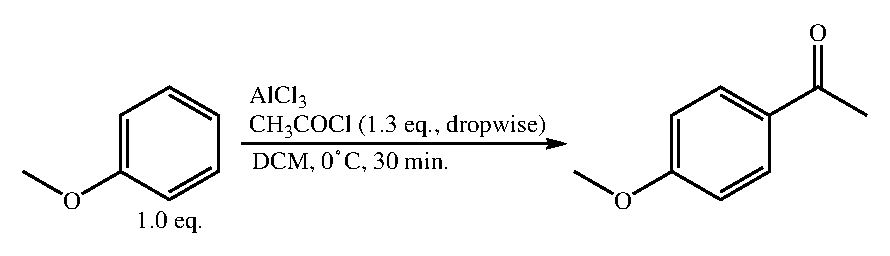
\includegraphics[scale=0.8]{schemes/acetylation.eps}
    \caption{Acetylation of anisole}
\end{figure}
\noindent\bf{Procedure.} Aluminum chloride (14 g) in DCM (15.0 mL) was added to a 250 mL two-necked round bottom flask and cooled to 0\degree C, followed by dropwise addition of acetyl chloride (9.27 g, 118 mmol) in DCM (10.0 mL) over 10 minutes with magnetic stirring. To the resulting mixture was added anisole (10.0 g, 93.9 mmol) dropwise over 30 minutes. Reaction progress was monitored using TLC (9:1 hexanes:EtOAc). When the reaction was completed, the reaction mixture was quenched in a beaker containing ice (\textasciitilde 30 mL) and hydrochloric acid (10 mL), then neutralized with saturated sodium bicarbonate. The resulting mixture was extracted with saturated sodium bicarbonate (2x1 vol.), washed with brine (1 vol.), dried with anhydrous sodium sulfate, and the solvent was evaporated under reduced pressure.

\noindent\bf{4-methoxyacetophenone:} Colorless solid/pale yellow liquid. Hexanes:EtOAC 9:1 R\textsubscript{f} = 0.53. \bf{$^1$H-NMR} (400 MHz): \textdelta\hspace{0mm} 2.539 (s, 3H), 3.849 (s, 3H), 6.907 - 6.929 (d, 2H) 7.912 - 7.934 (d, 2H). \bf{IR} (neat): 2970, 2842, 1671, 1597, 1509, 1417, 1357, 1247, 1169, 1025, 956, 832 cm$^{-1}$. \bf{UV-Vis:} \textlambda\textsubscript{max} = 270 nm. \bf{Yield:} (9.247 g, 66.24\%).

\begin{figure}[H]
    \centering
    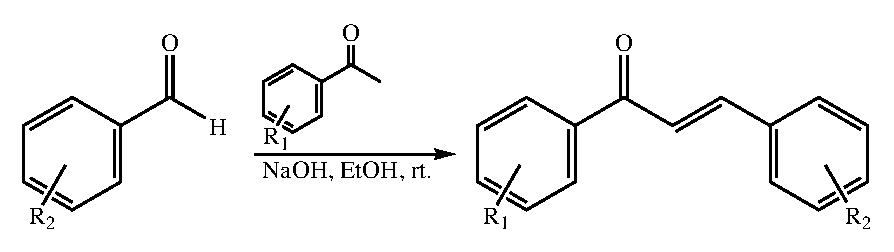
\includegraphics[scale=0.8]{schemes/chalcone.eps}
    \caption{Aldol condensation of benzaldehyde and acetophenone}
\end{figure}
\noindent\bf{Prodedure.} To a 150 mL Erlenmeyer flask was added 3-nitrobenzaldehyde (0.76 g, 5.0 mmol) followed by the acetophenone (5.0 mmol) and 95\% EtOH (4 mL). Once all the solid was dissolved, NaOH solution (0.5 mL) was added with constant stirring until the mixture solidified. After 5 minutes of additional stirring, the resulting solid was quenched with ice water (\textasciitilde 10 mL), filtered by vacuum, and recrystallized from hot 95\% EtOH.

\noindent\bf{3-(3-nitrophenyl)-1-phenylprop-2-en-1-one:} light green powder. \bf{$^1$H-NMR} (400 MHz): \textdelta\hspace{0mm} 7.527 - 7.564 (t, 2H), 7.608 - 7.644 (t, 2H), 7.648 - 7.684 (d, 1H), 7.823 - 7.863 (d, 1H), 7.922 - 7.941 (d, 1H), 8.043 - 8.067 (d, 2H), 8.259 - 8.282 (dq, 1H), 8.519 - 8.528 (t, 1H). \bf{IR} (neat): 3071, 1659, 1606, 1526, 1446, 1349, 1217 cm$^{-1}$. \bf{UV-Vis:} \textlambda\textsubscript{max} = 237 nm. \bf{Yield:} (1.989 g, 158.3\%)

\noindent\bf{1-(4-methoxyphenyl)-3-(3-nitrophenyl)prop-2-en-1-one:} blue-green powder. \bf{$^1$H-NMR} (400 MHz): \textdelta\hspace{0mm} 3.914 (s, 3H), 7.005 - 7.027 (d, 2H), 7.596 - 7.636 (t, 1H), 7.648 - 7.687 (d, 1H), 7.806 - 7.846 (d, 1H), 7.906 - 7.925 (d, 1H), 8.061 - 8.083 (d, 2H), 8.239 - 8.268 (dq, 1H), 8.515 - 8.524 (t, 1H). \bf{IR} (neat): 3357, 2981, 2888, 1662, 1595, 1521, 1339, 1258, 1167 cm$^{-1}$. \bf{UV-Vis:} \textlambda\textsubscript{max} = 322 nm. \bf{Yield:} (847 mg, 59.92\%)

\newpage
\subsection*{REFERENCES}
\bibliography{references}

\newpage
\subsection*{APPENDIX A: SPECTRA}
%%% NMR SPECTRA %%%
\begin{figure}[h]
    \centering
    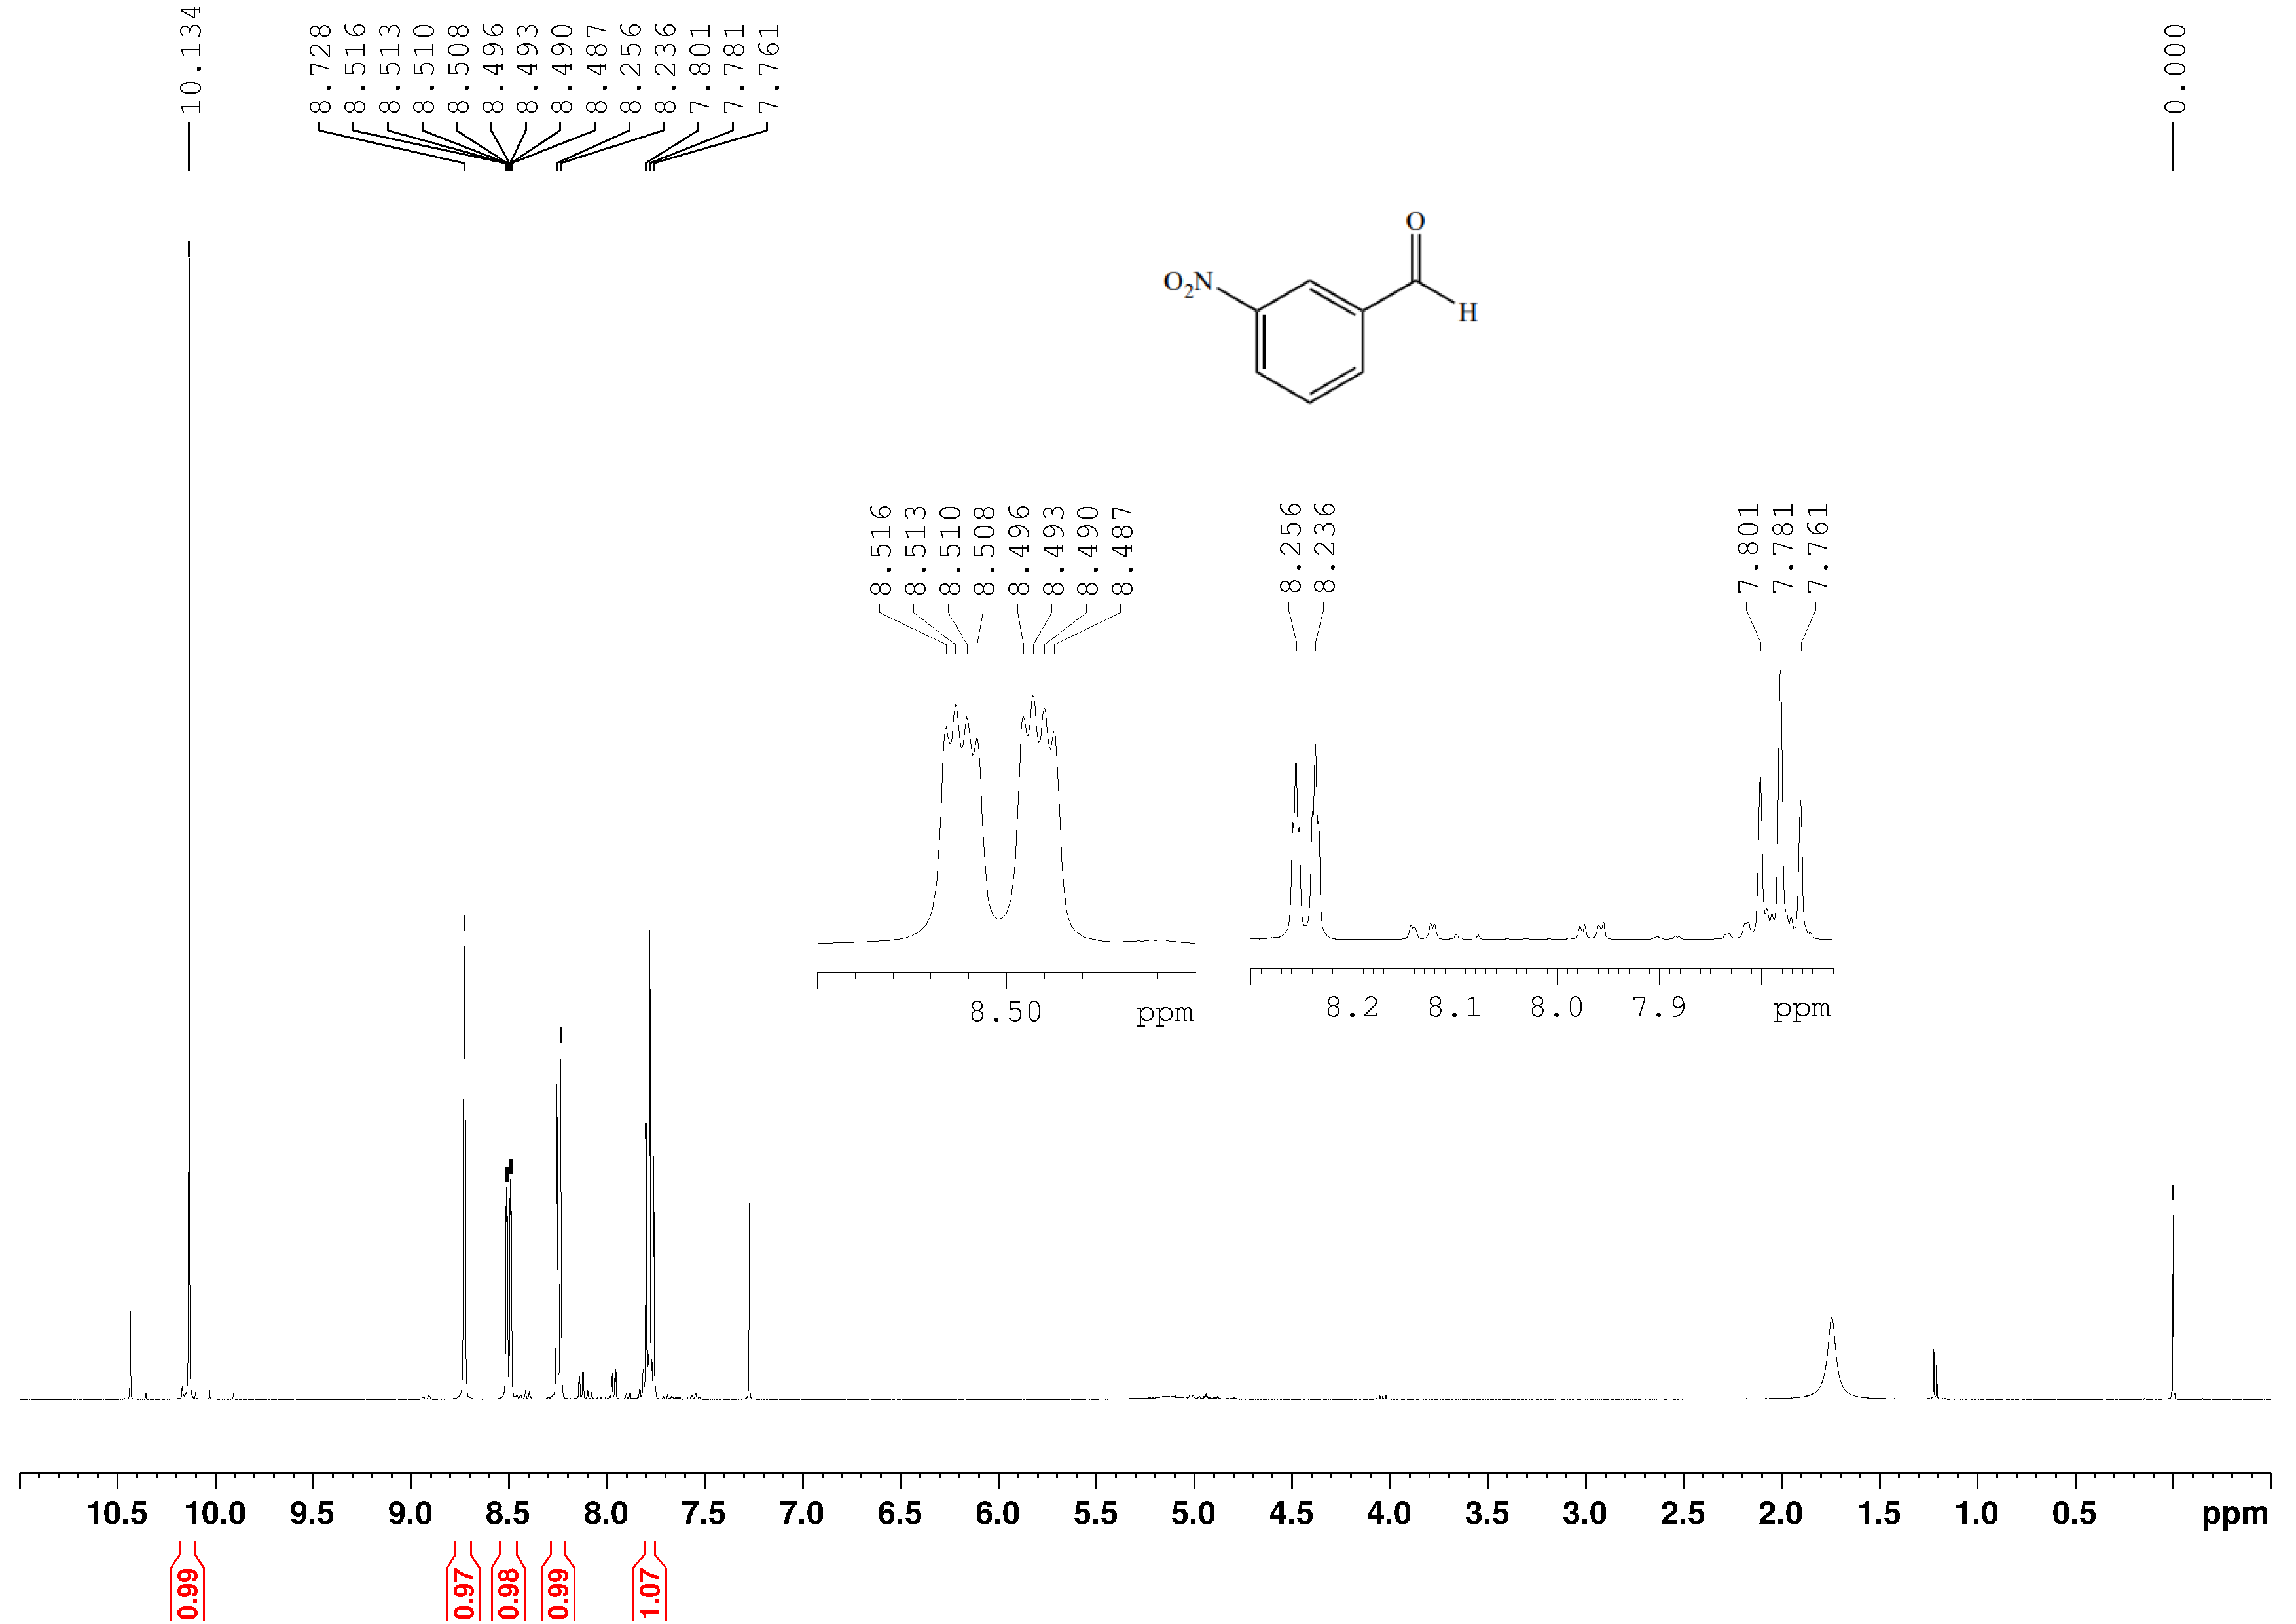
\includegraphics[scale=0.105]{spectra/nmr4.1.png}
    \caption{3-nitrobenzaldehyde NMR}
\end{figure}
\begin{figure}[h!]
    \centering
    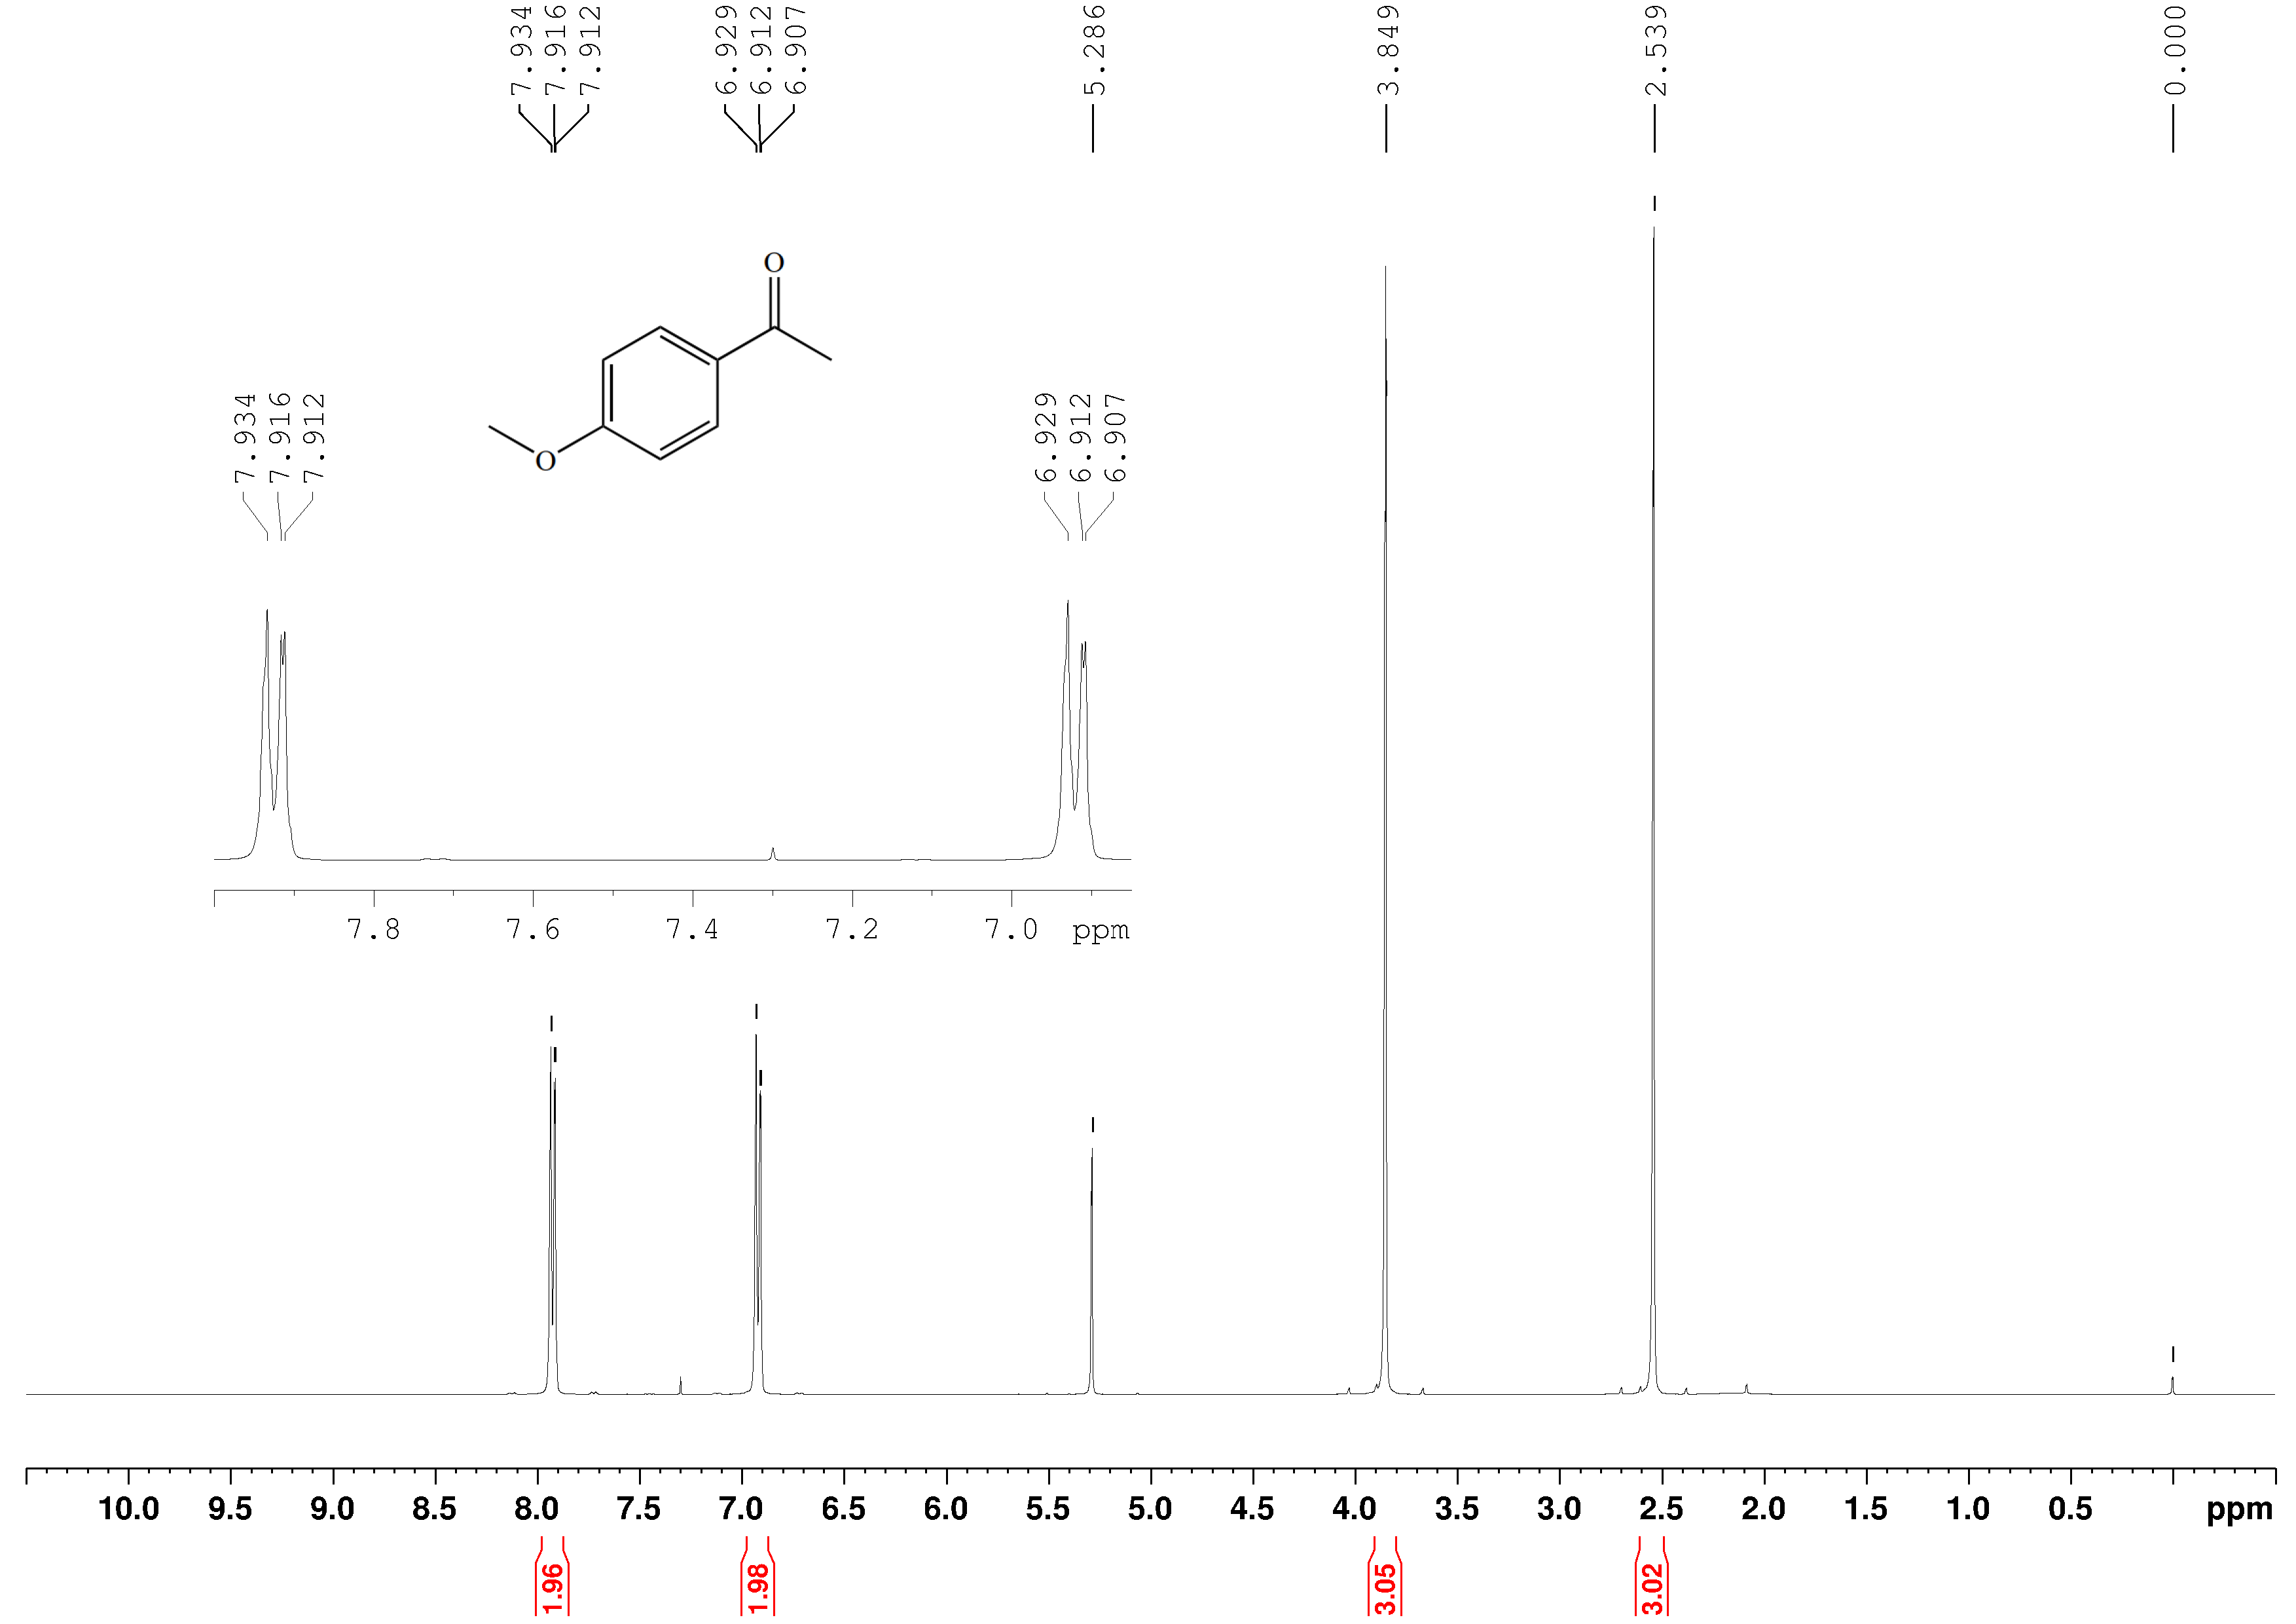
\includegraphics[scale=0.105]{spectra/nmr5.1.png}
    \caption{1-(4-methoxyphenyl)ethan-1-one NMR}
\end{figure}

\newpage
\begin{figure}[H]
    \centering
    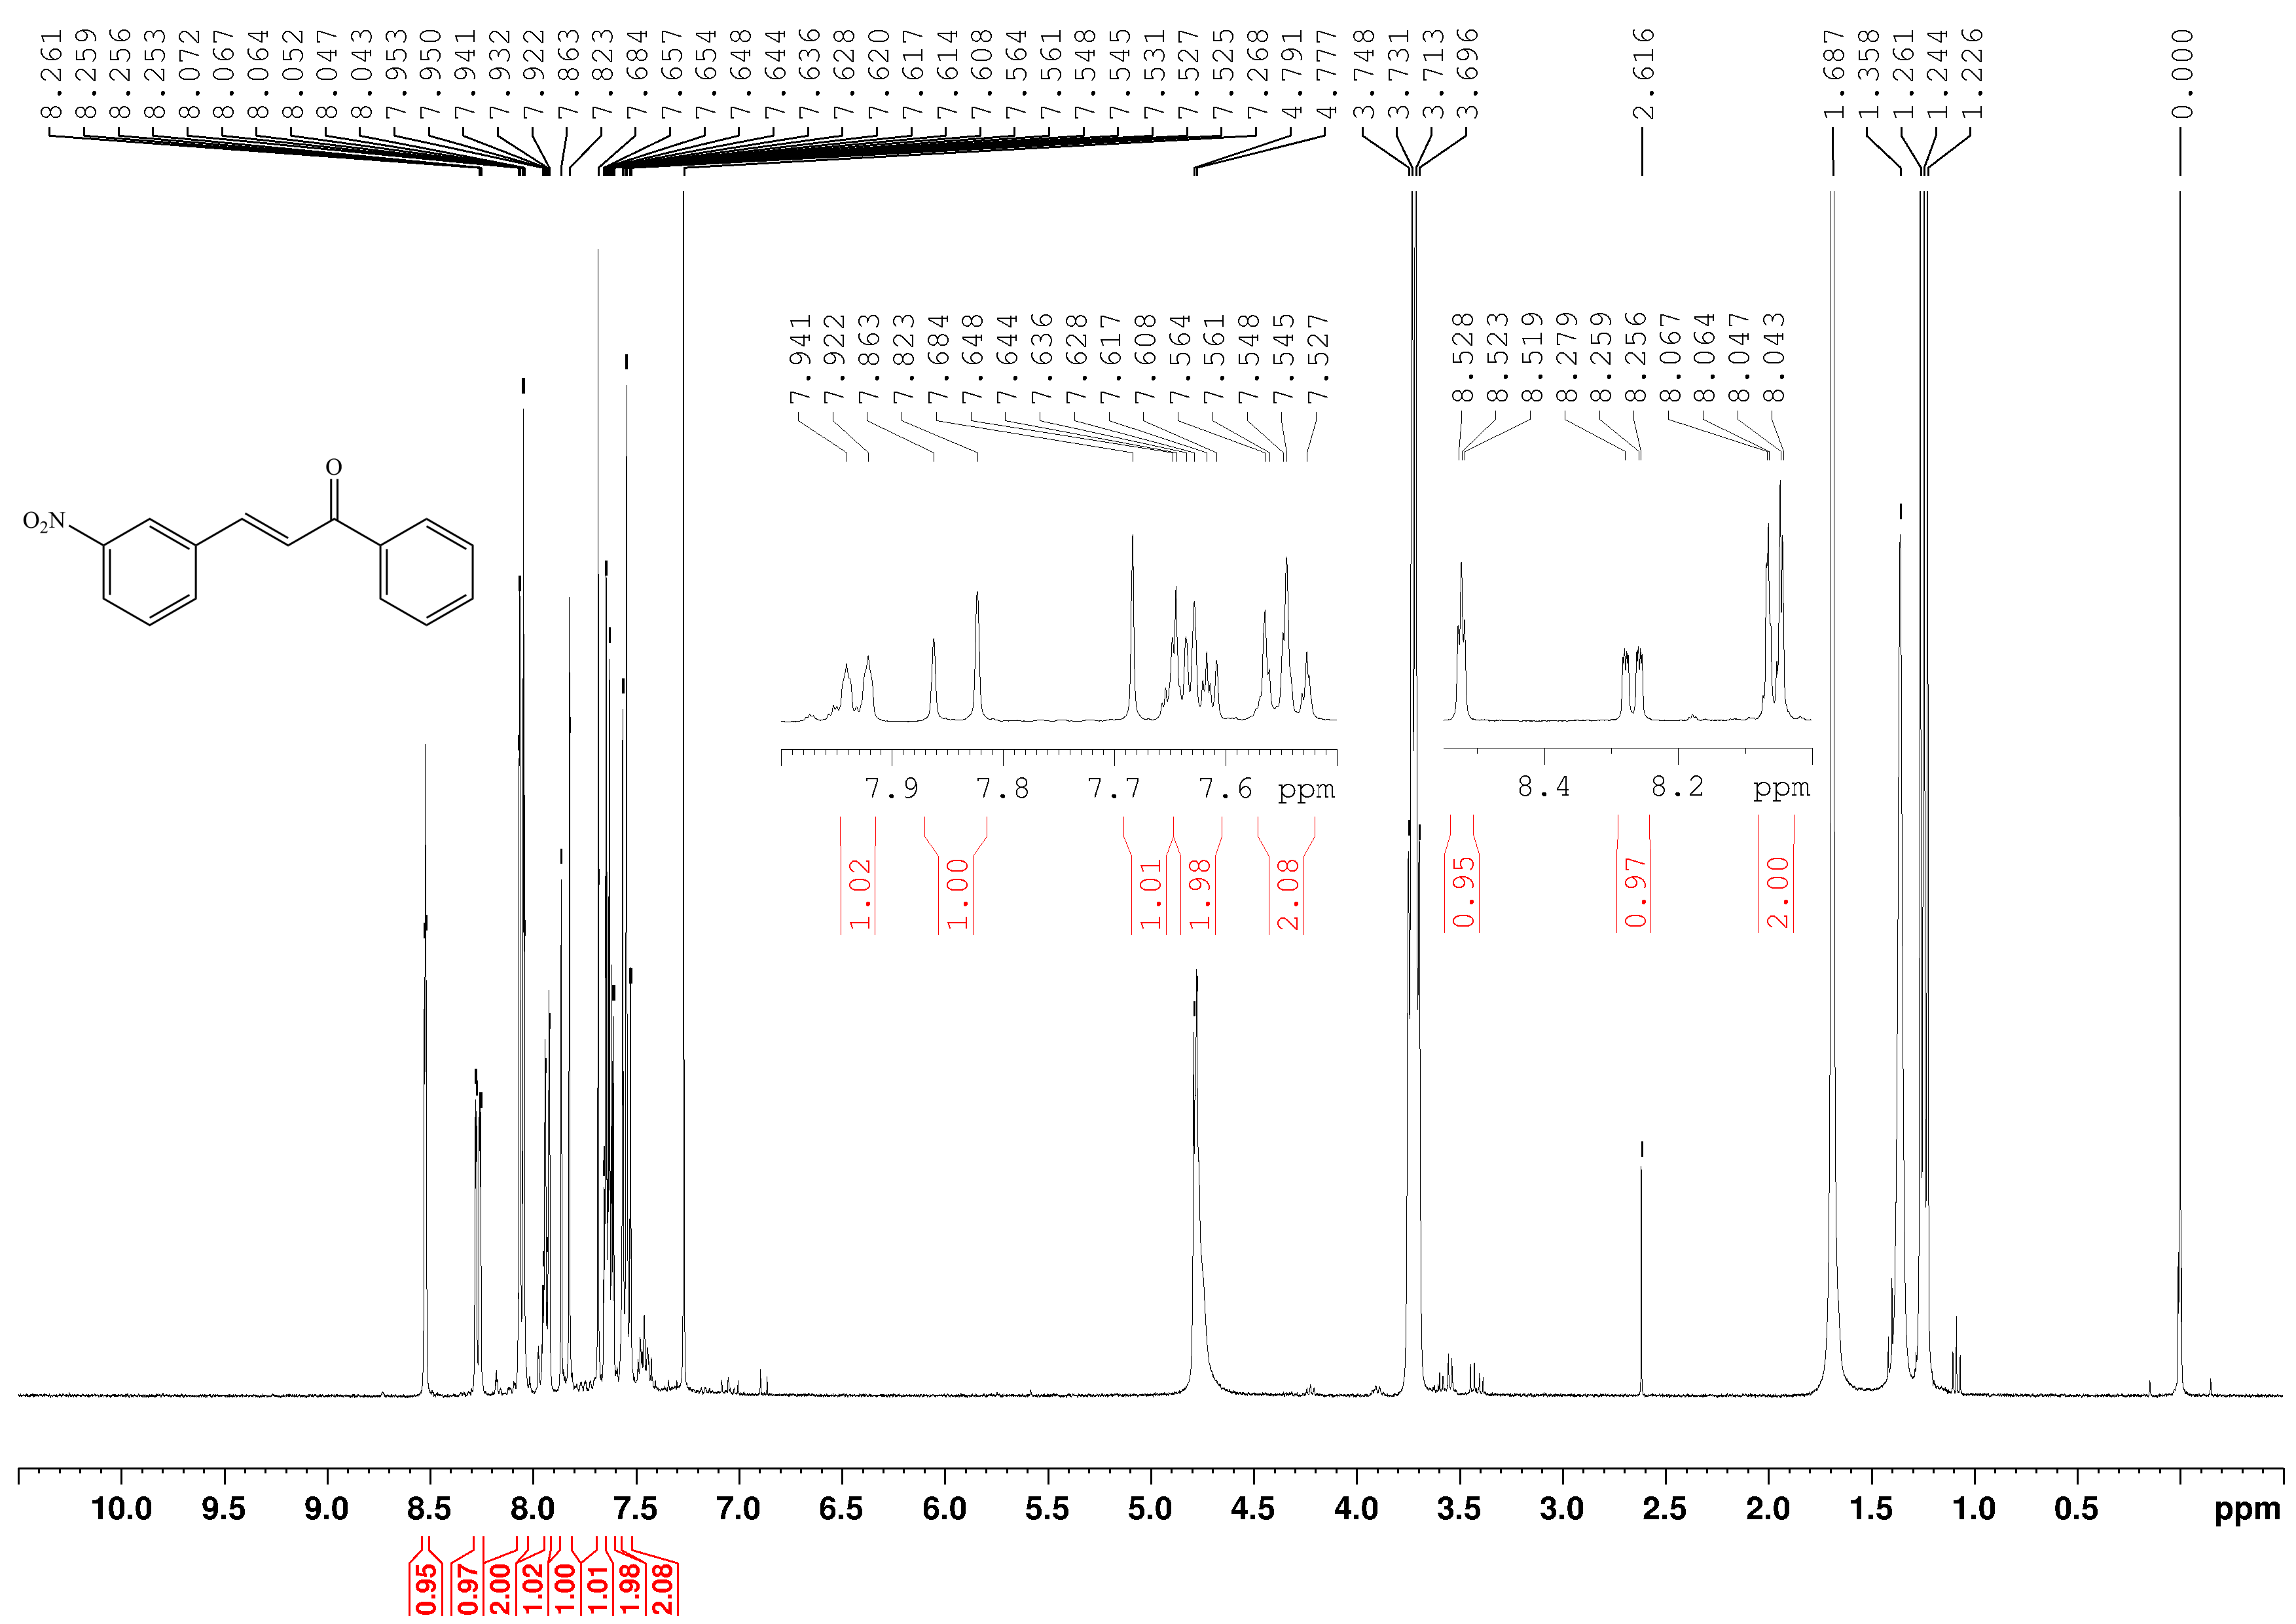
\includegraphics[scale=0.105]{spectra/nmr7.1.png}
    \caption{3-(3-nitrophenyl)-1-phenylprop-2-en-1-one NMR}
\end{figure}
\begin{figure}[H]
    \centering
    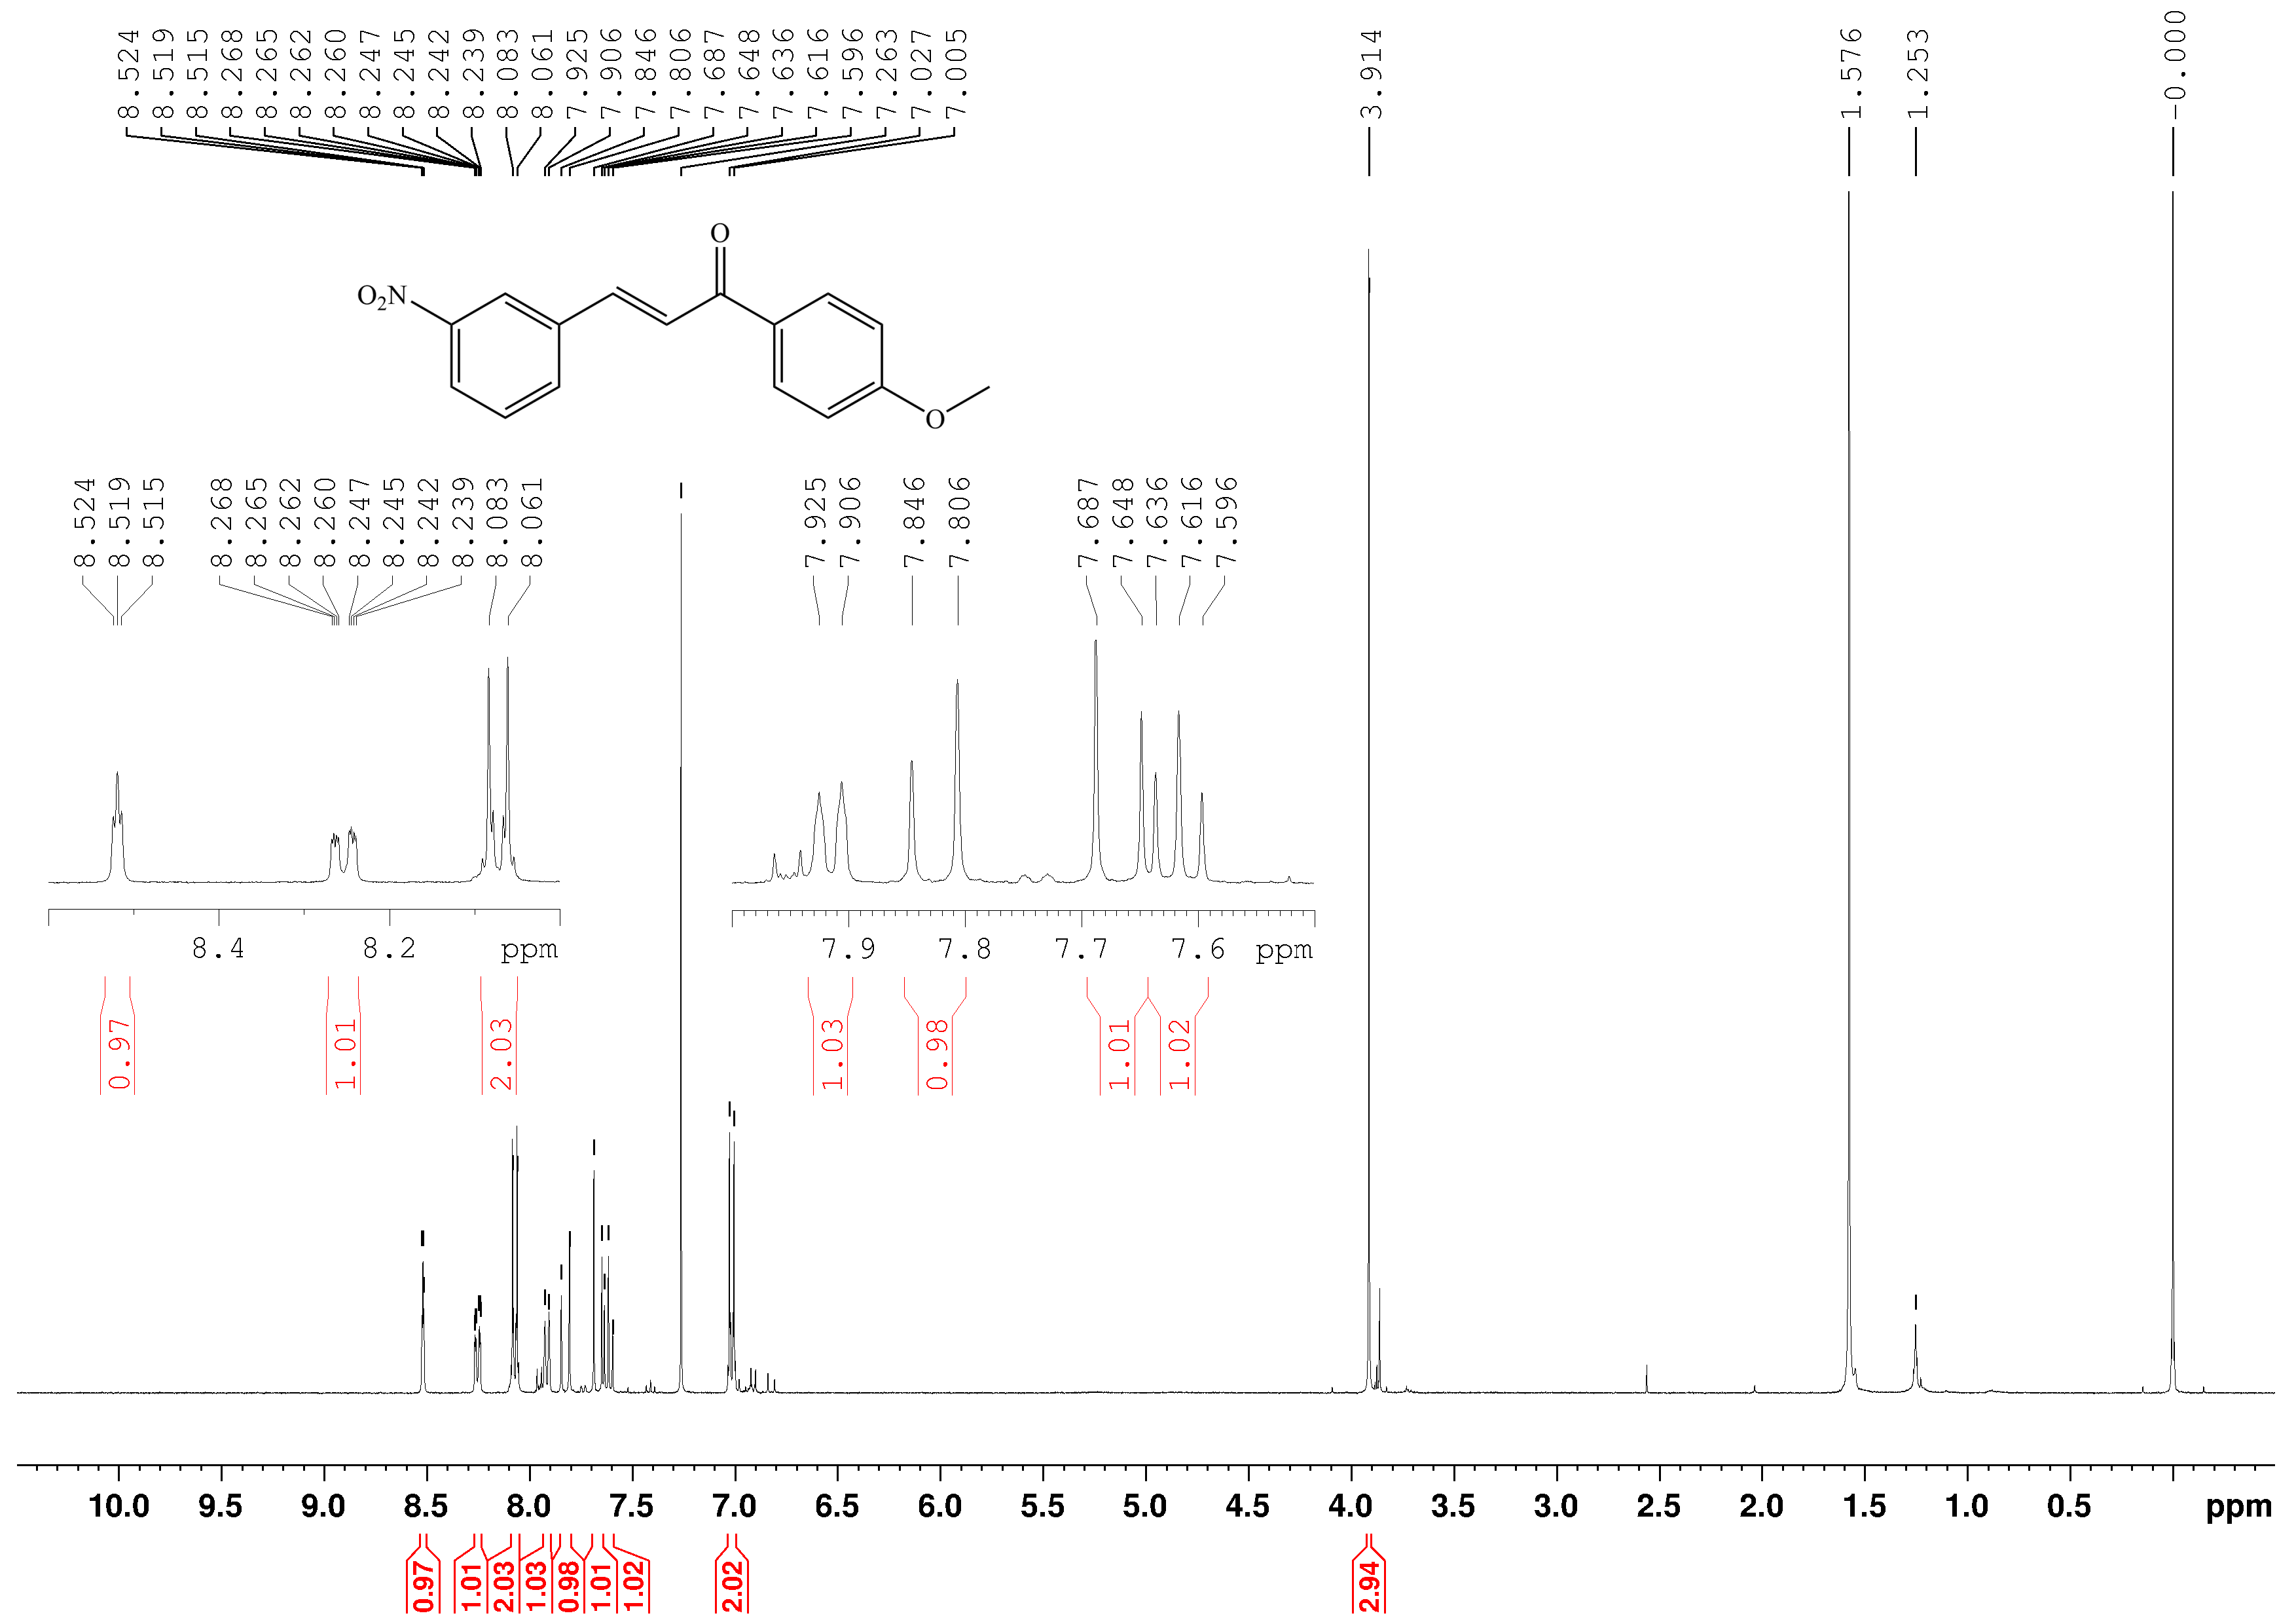
\includegraphics[scale=0.105]{spectra/nmr7.2.png}
    \caption{1-(4-methoxyphenyl)-3-(3-nitrophenyl)prop-2-en-1-one NMR}
\end{figure}

\newpage
%%% IR SPECTRA %%%
\begin{figure}[H]
    \centering
    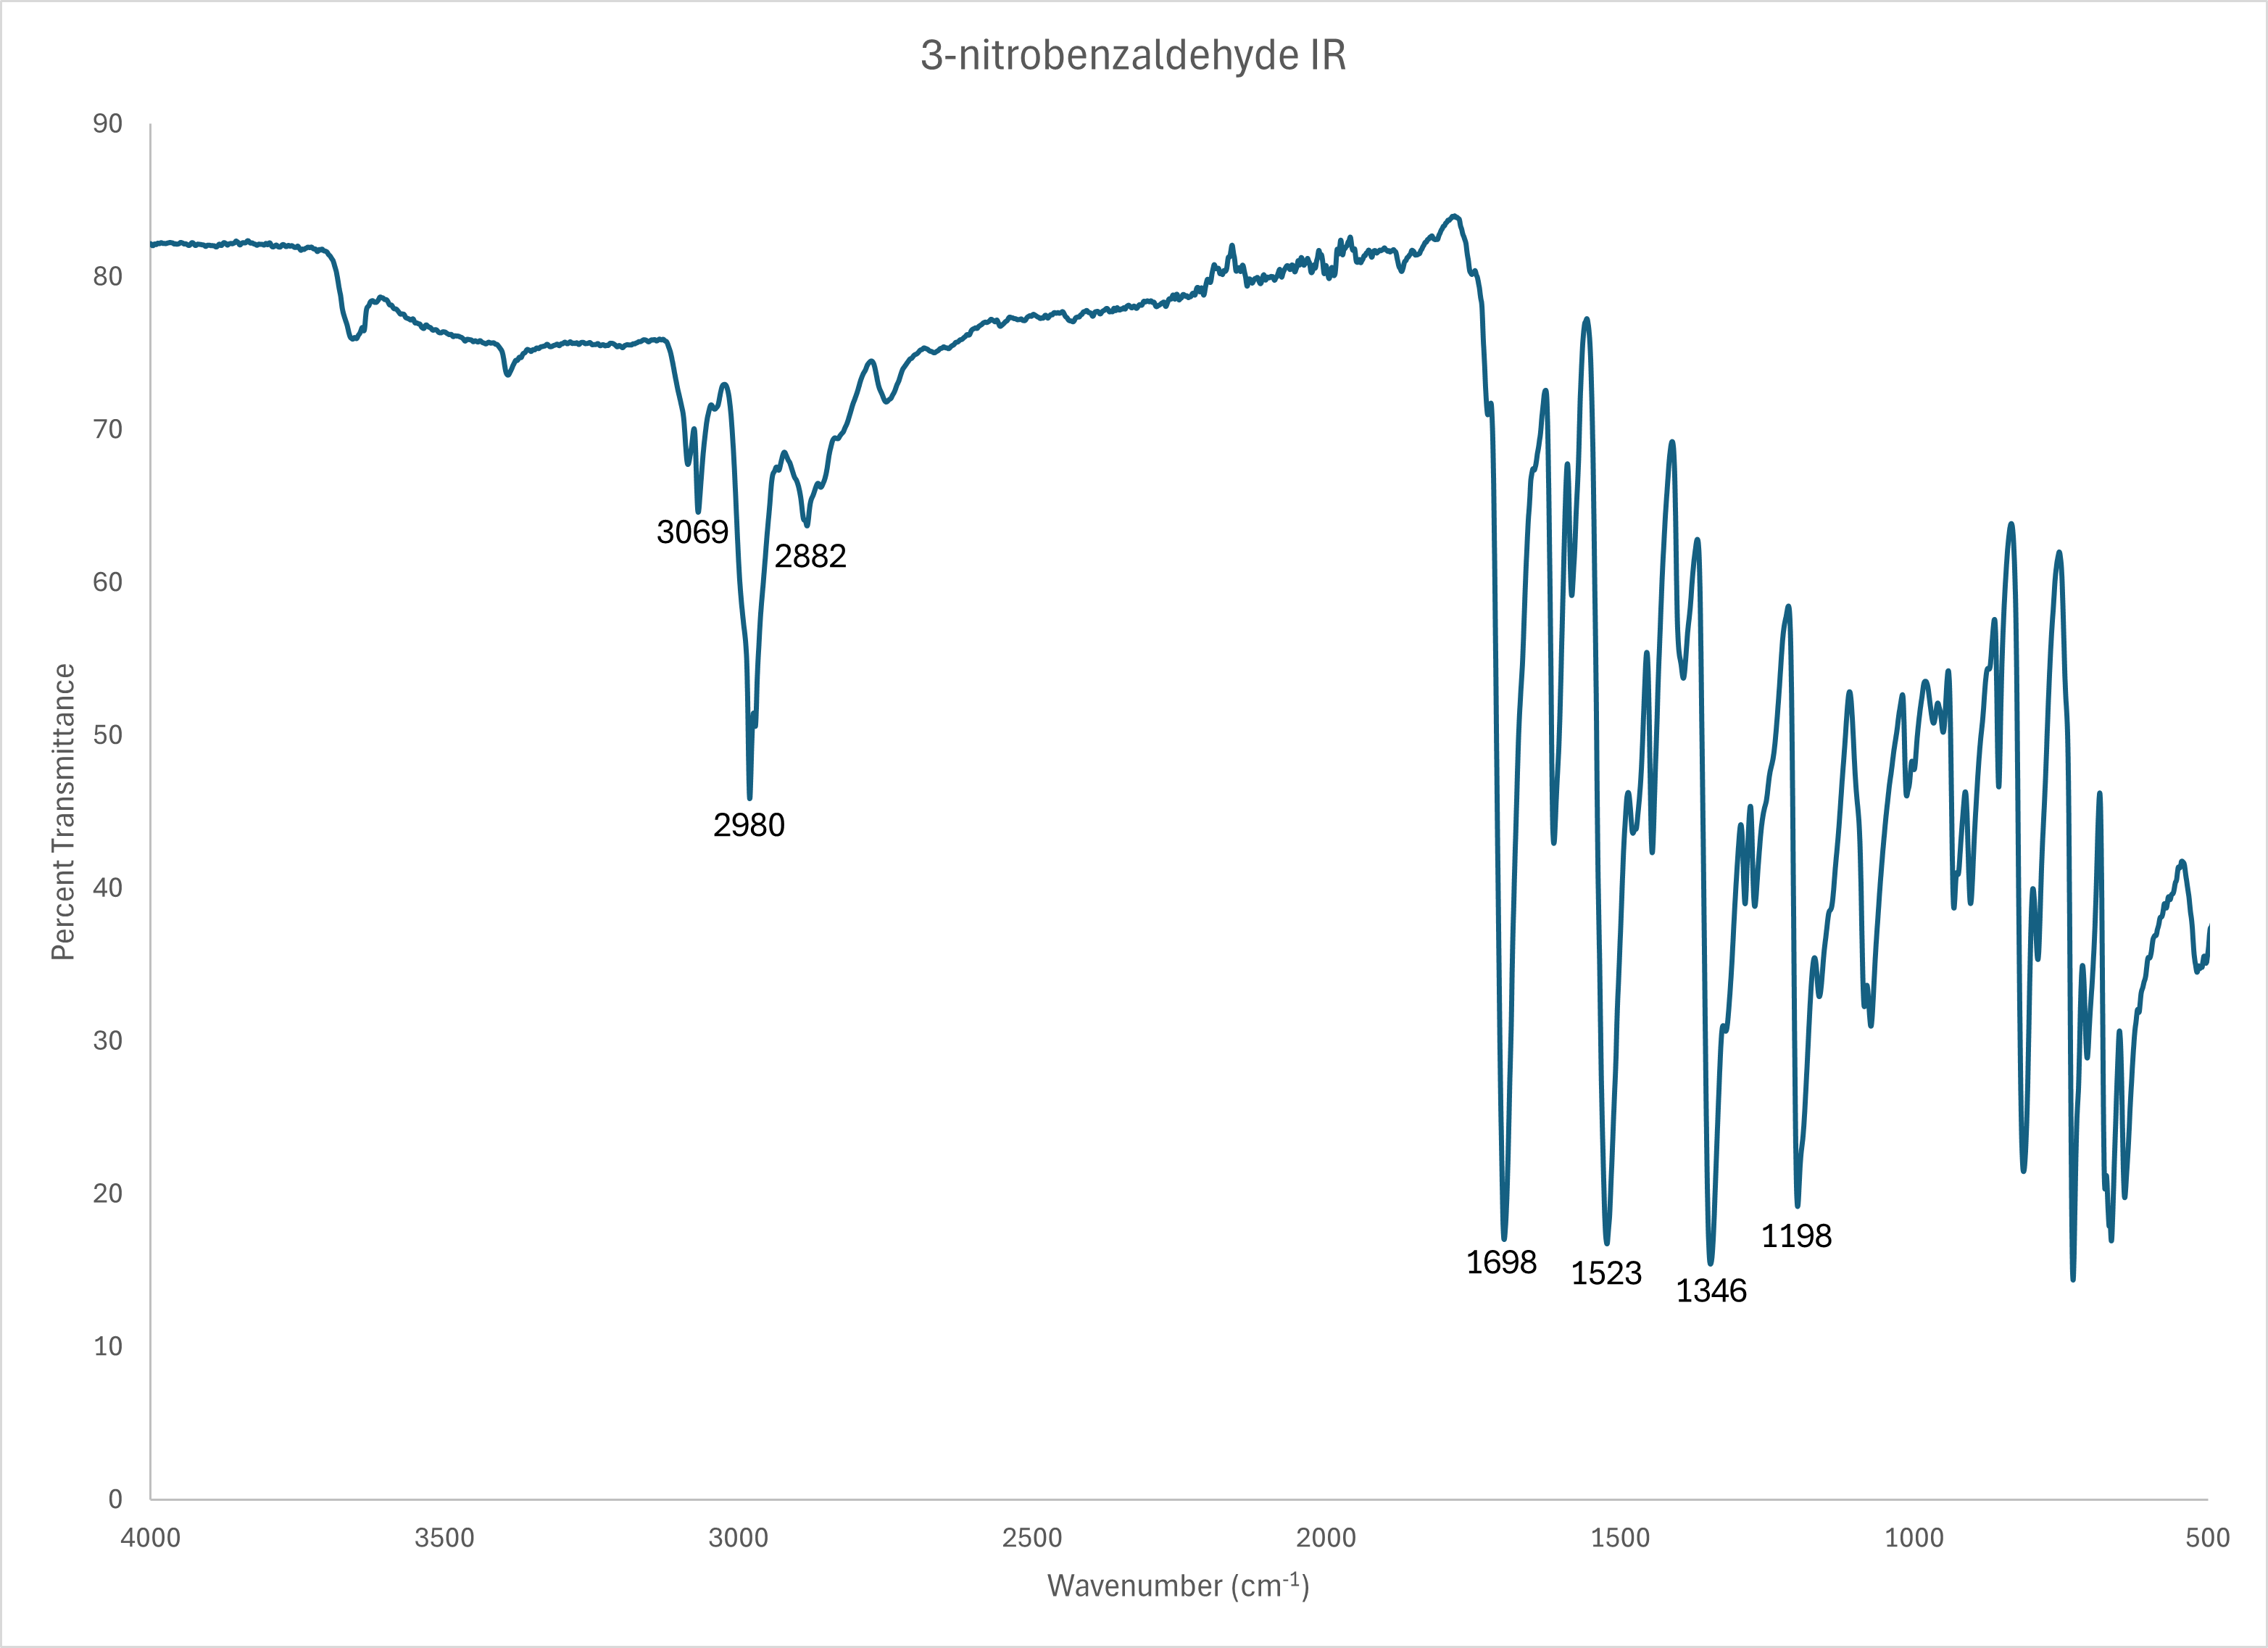
\includegraphics[scale=0.234]{spectra/ir4.1.png}
    \caption{3-nitrobenzaldehyde IR}
\end{figure}
\begin{figure}[H]
    \centering
    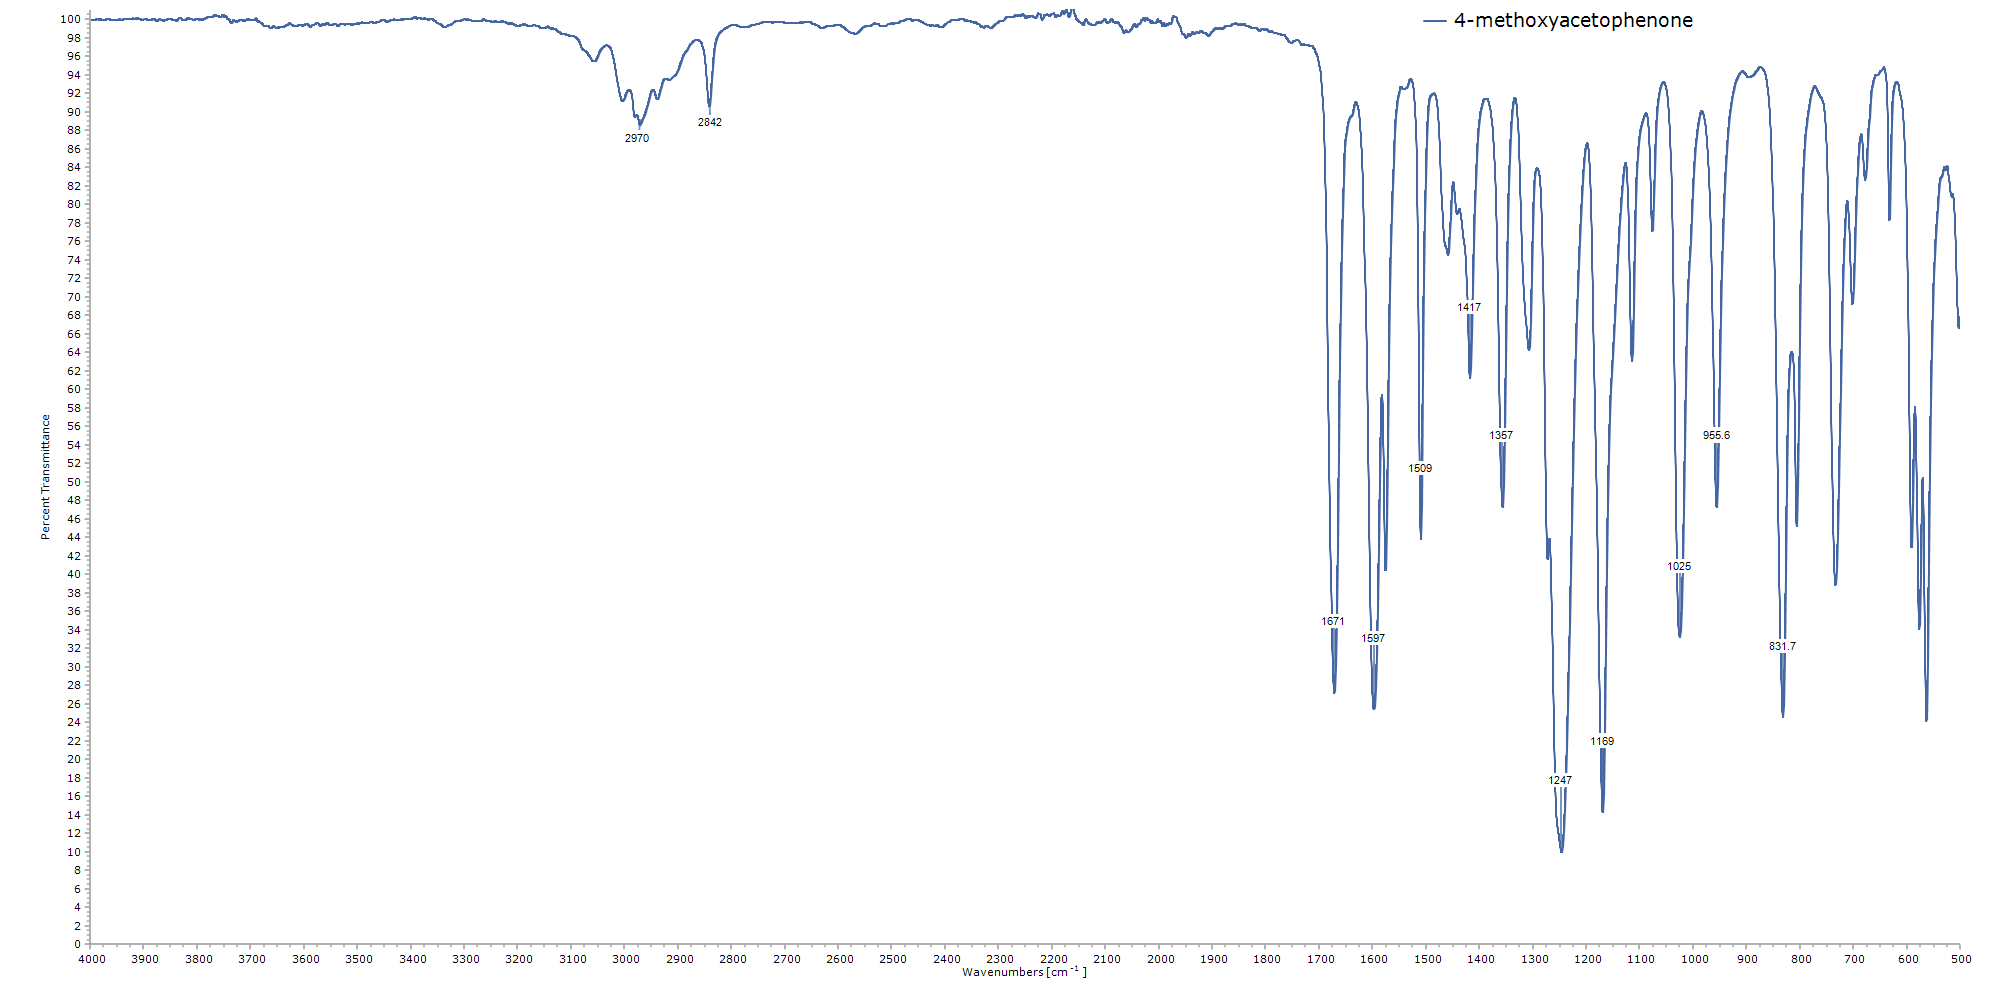
\includegraphics[scale=0.234]{spectra/ir5.1.png}
    \caption{1-(4-methoxyphenyl)ethan-1-one IR}
\end{figure}

\newpage
\begin{figure}[H]
    \centering
    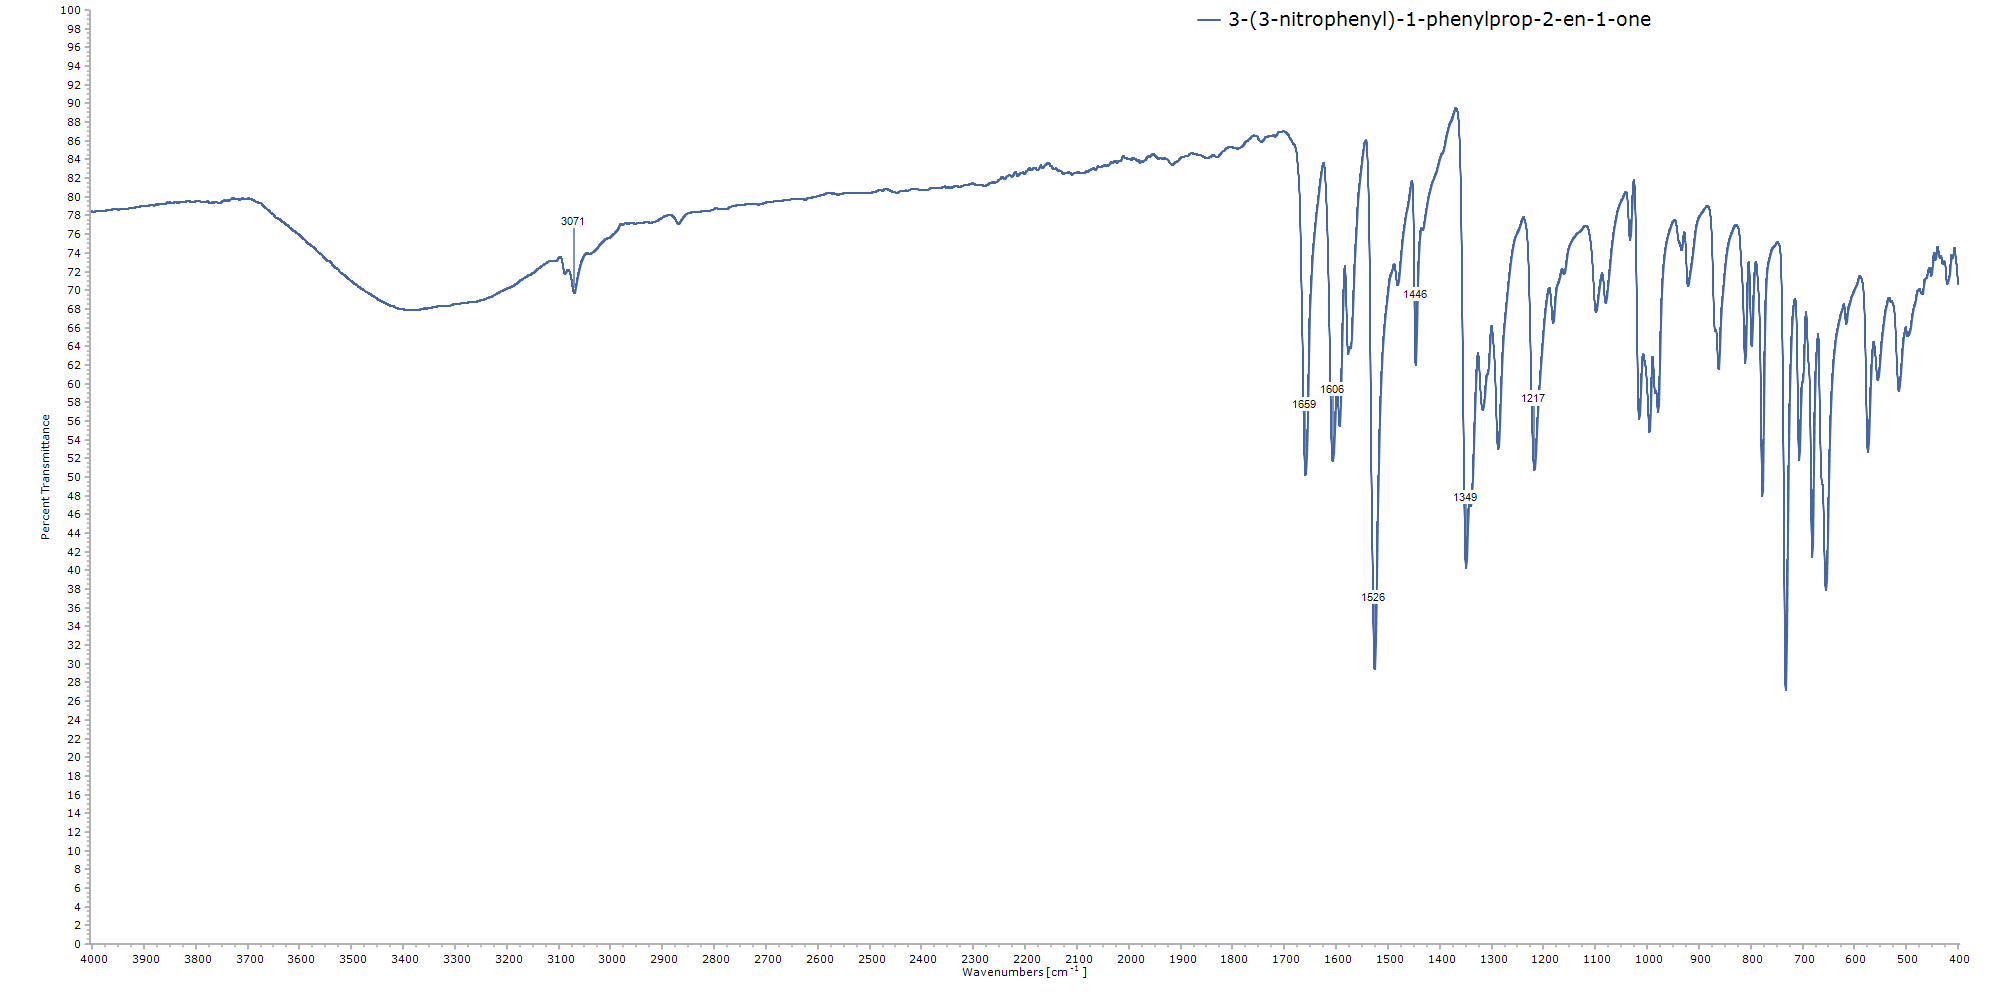
\includegraphics[scale=0.234]{spectra/ir7.1.png}
    \caption{3-(3-nitrophenyl)-1-phenylprop-2-en-1-one IR}
\end{figure}
\begin{figure}[H]
    \centering
    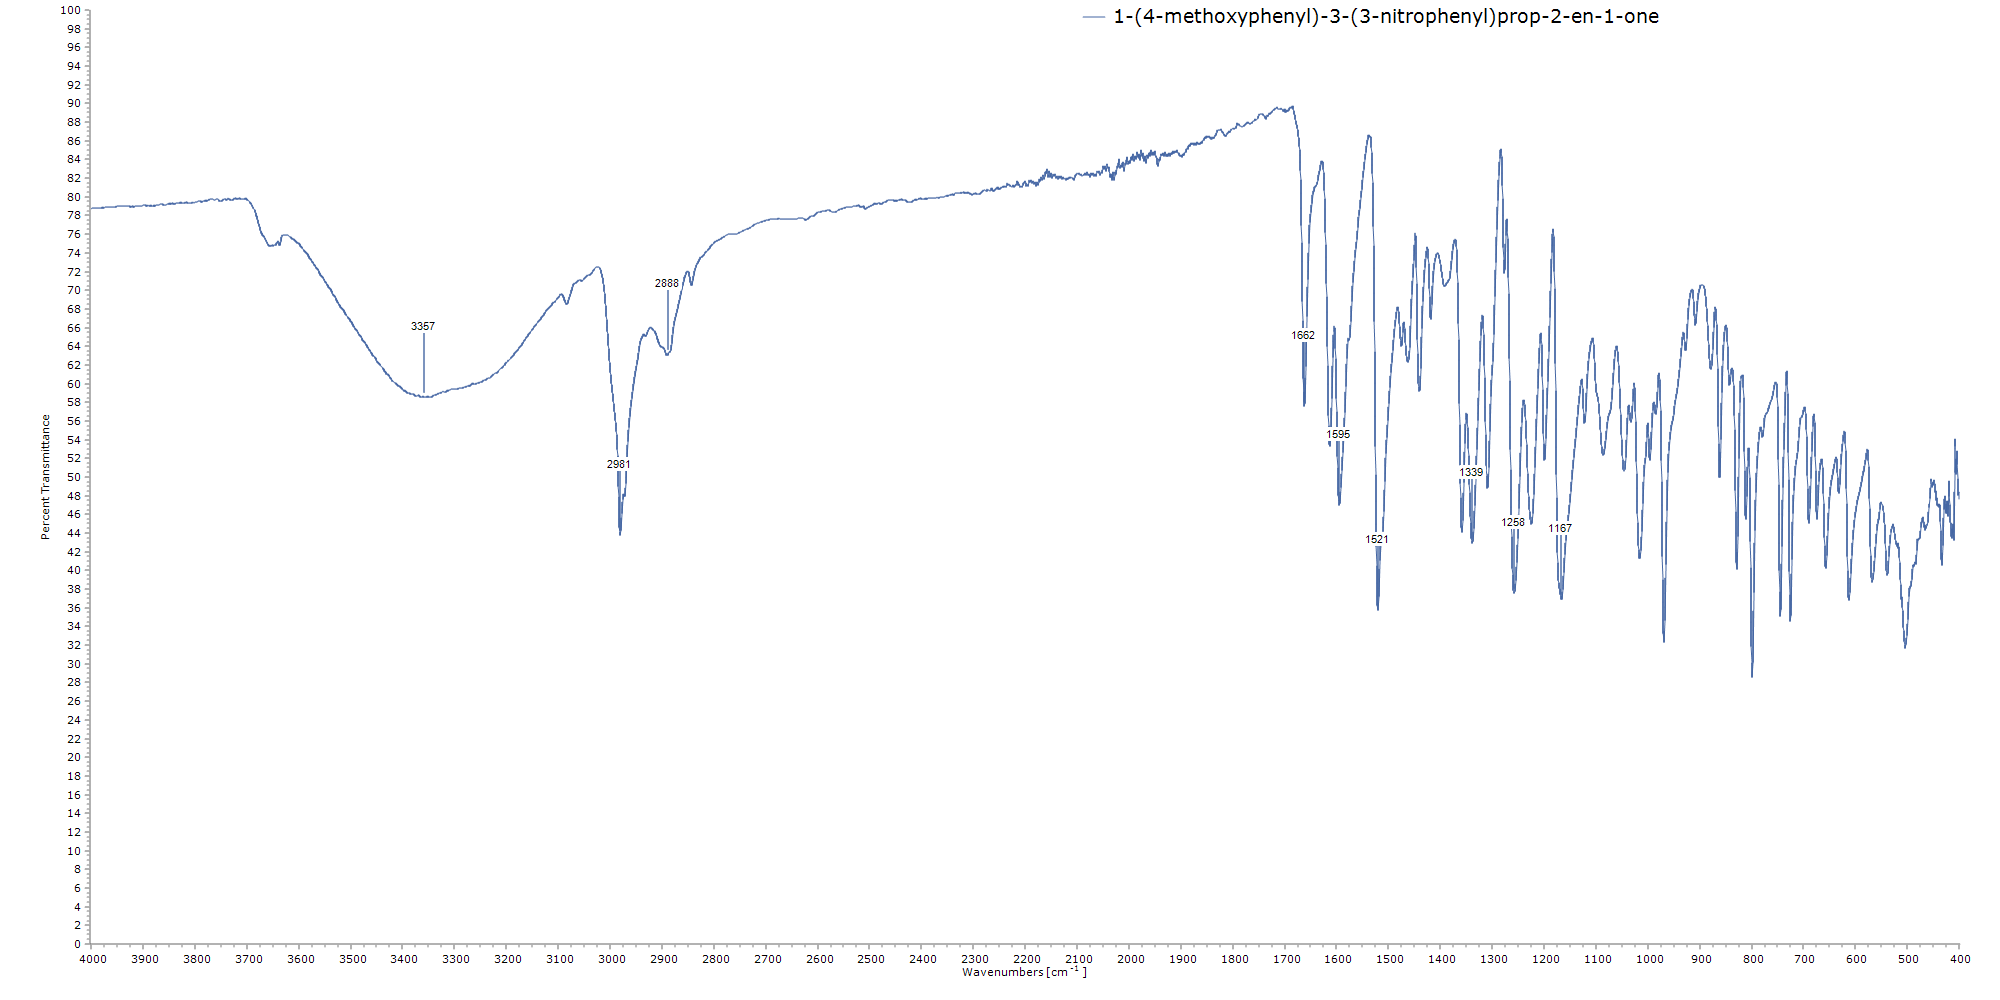
\includegraphics[scale=0.234]{spectra/ir7.2.png}
    \caption{1-(4-methoxyphenyl)-3-(3-nitrophenyl)prop-2-en-1-one IR}
\end{figure}

\newpage
%%% UV-VIS SPECTRA %%%
\begin{figure}[H]
    \centering
    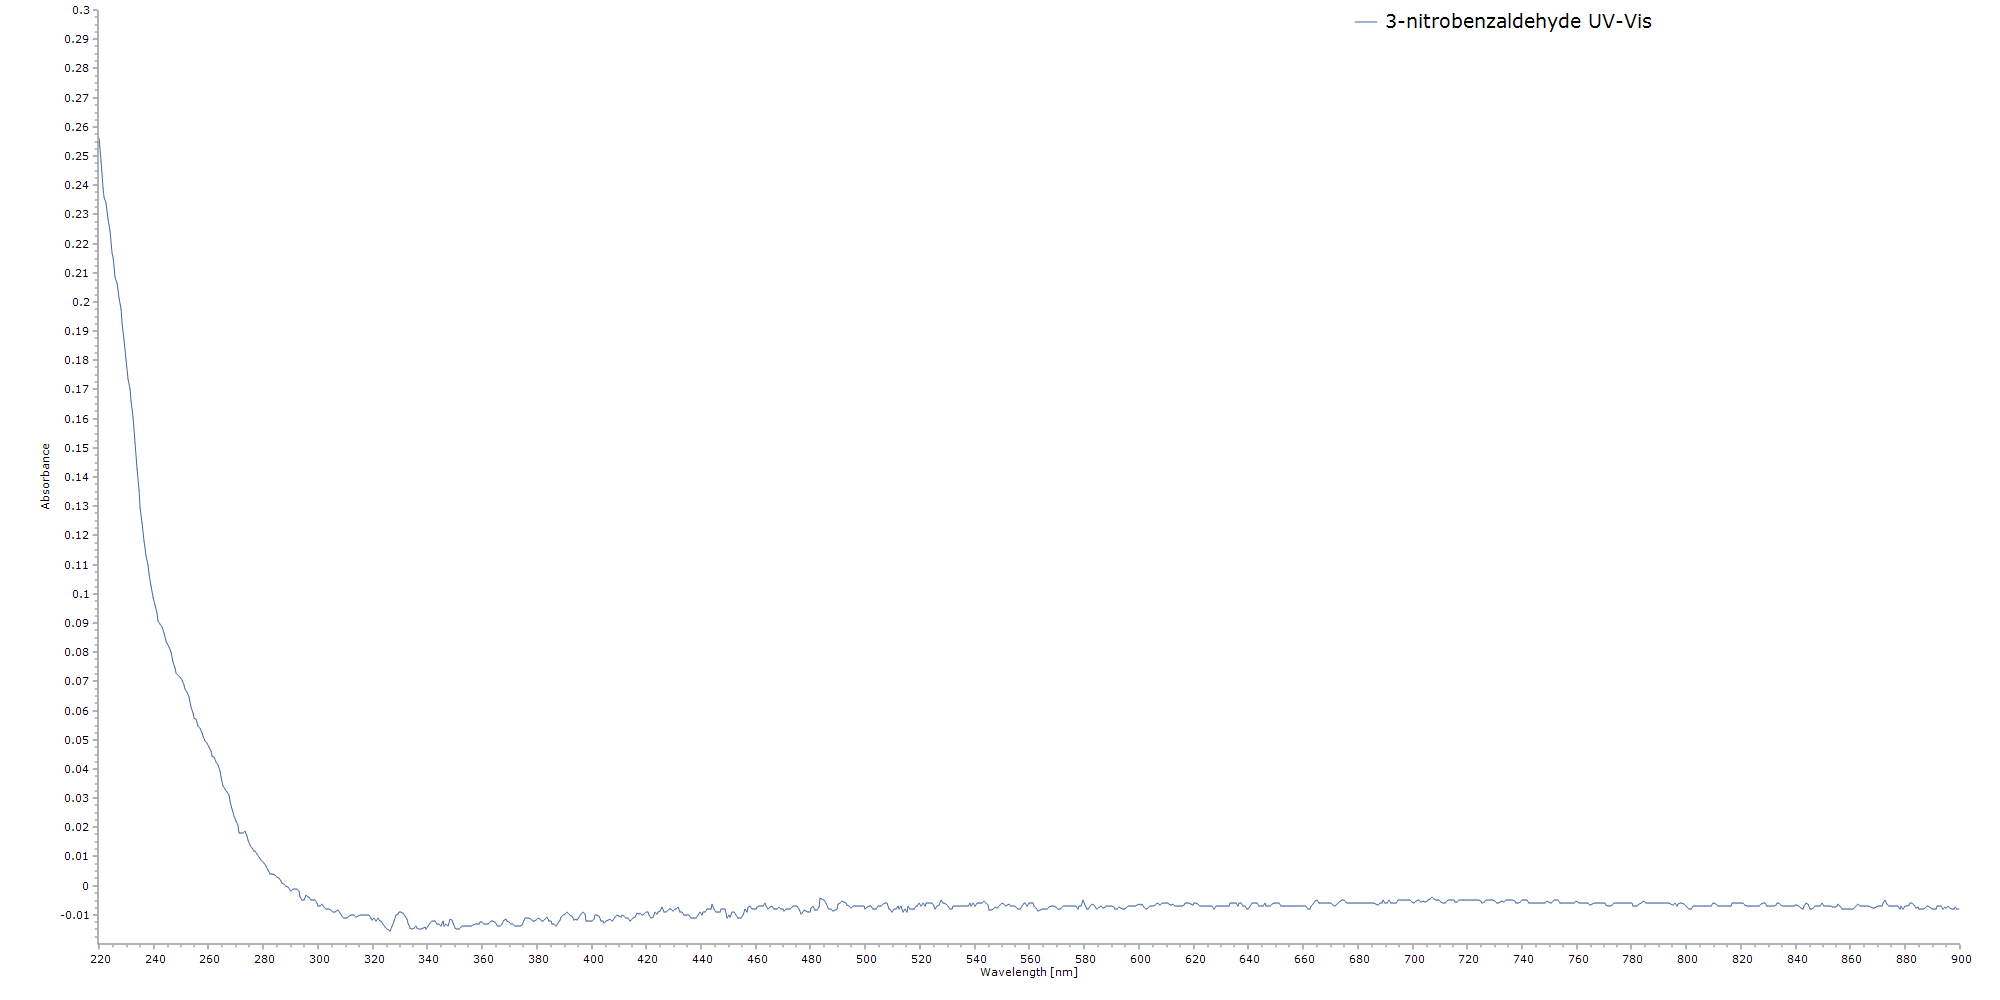
\includegraphics[scale=0.234]{spectra/uvvis4.1.png}
    \caption{3-nitrobenzaldehyde UV-Vis}    
\end{figure}
\begin{figure}[H]
    \centering
    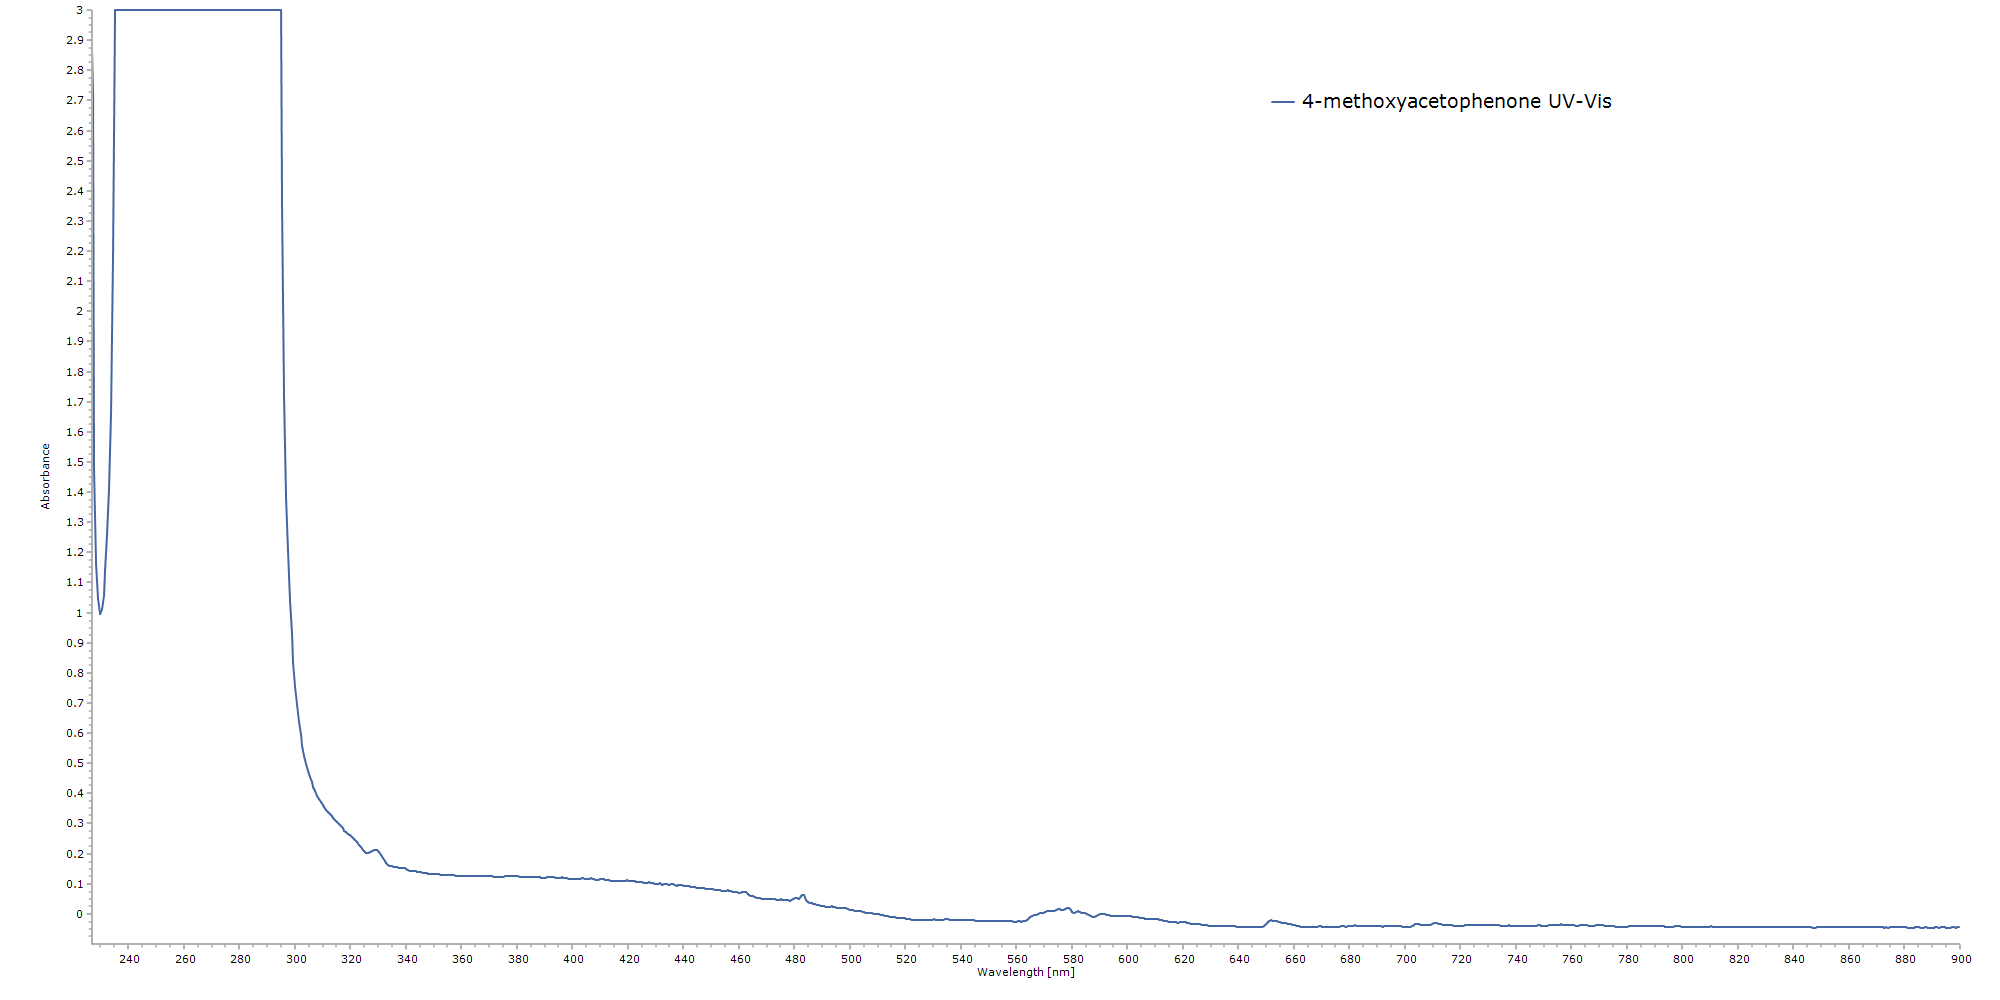
\includegraphics[scale=0.234]{spectra/uvvis5.1.png}
    \caption{1-(4-methoxyphenyl)ethan-1-one UV-Vis}    
\end{figure}

\newpage
\begin{figure}[H]
    \centering
    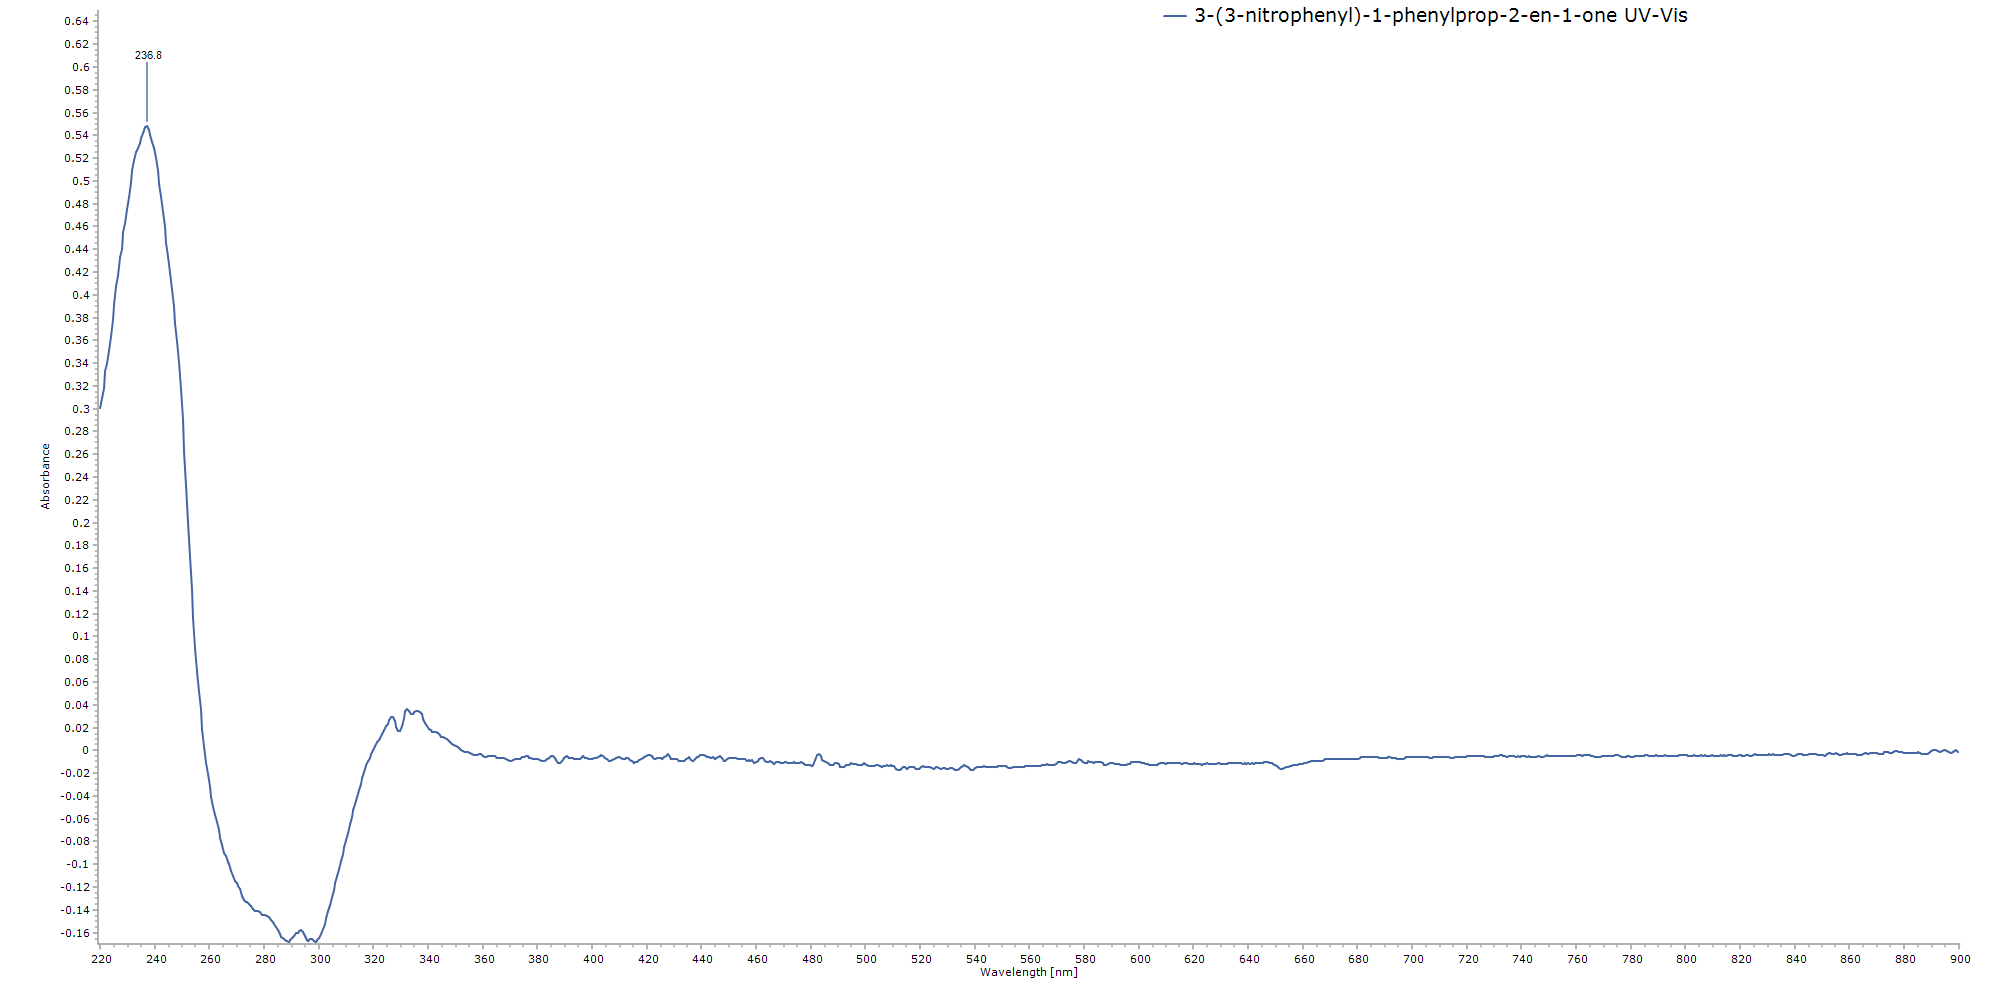
\includegraphics[scale=0.234]{spectra/uvvis7.1.png}
    \caption{3-(3-nitrophenyl)-1-phenylprop-2-en-1-one UV-Vis}
\end{figure}
\begin{figure}[H]
    \centering
    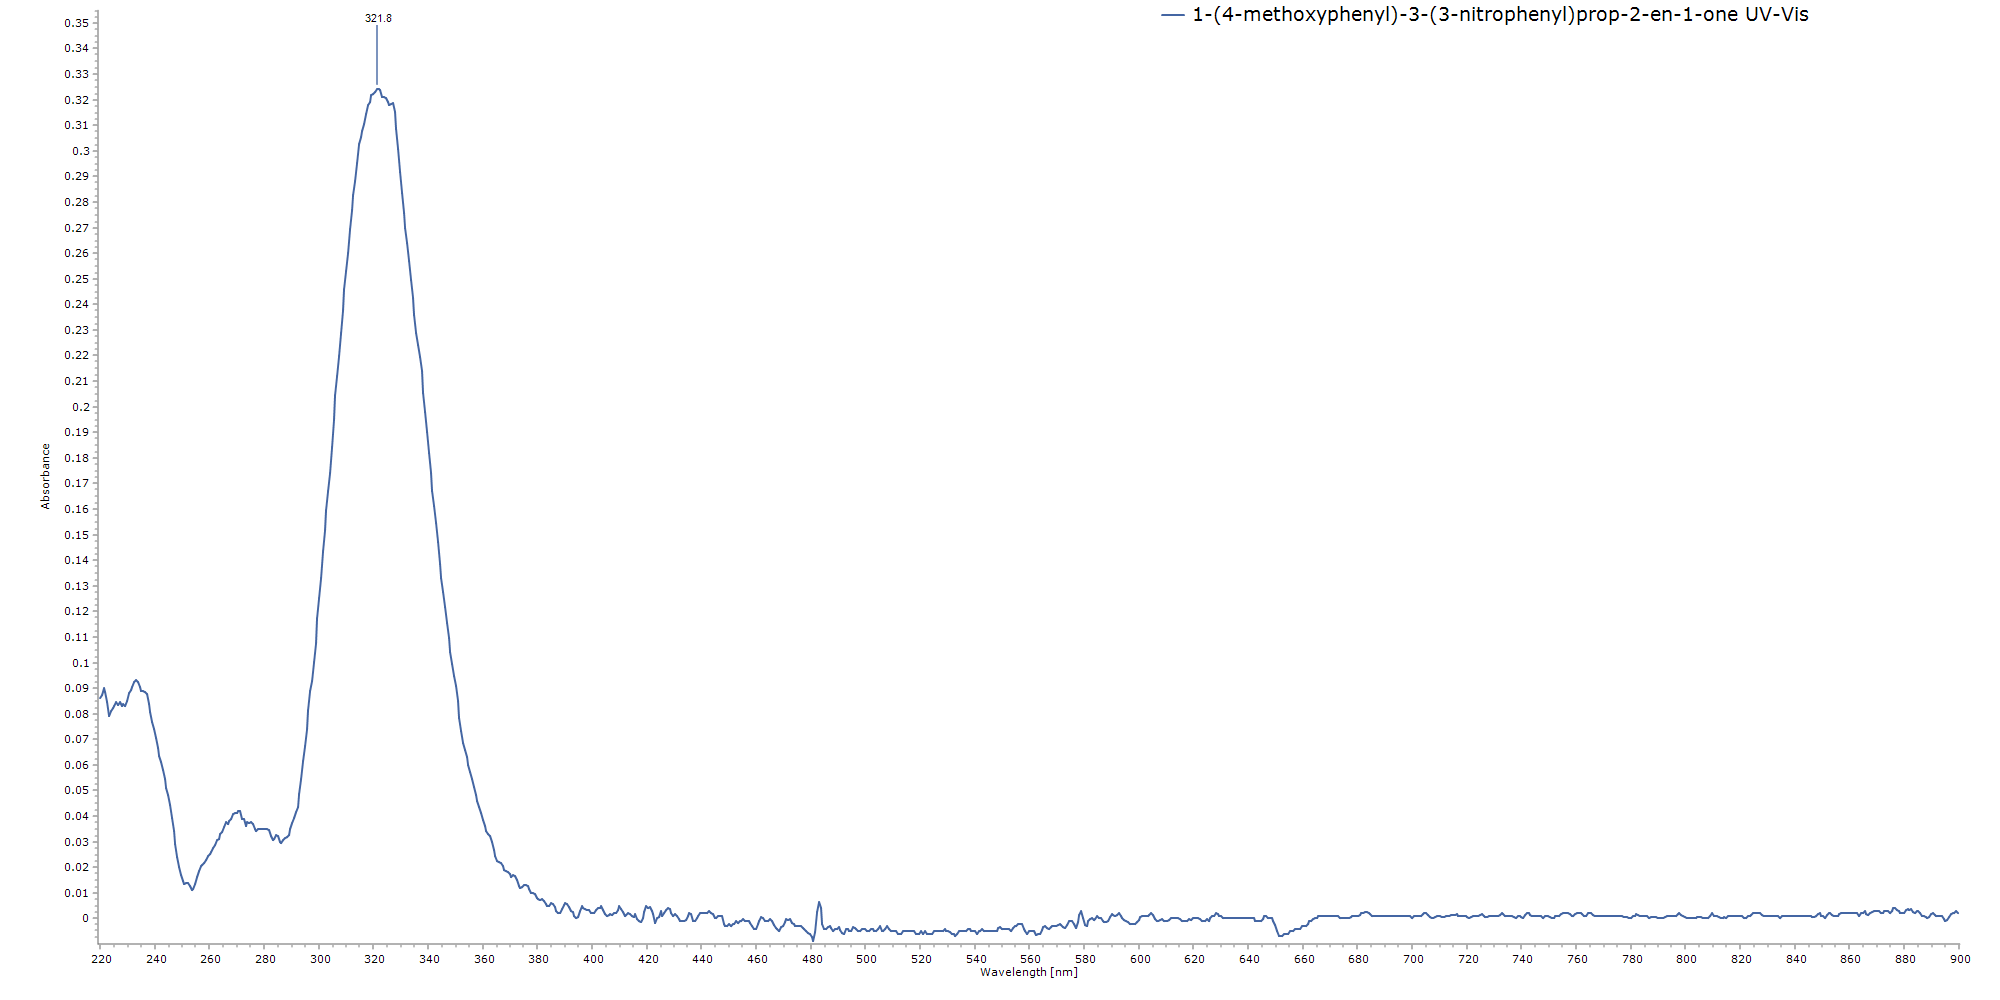
\includegraphics[scale=0.234]{spectra/uvvis7.2.png}
    \caption{1-(4-methoxyphenyl)-3-(3-nitrophenyl)prop-2-en-1-one UV-Vis}
\end{figure}

\newpage
\subsection*{APPENDIX B: MECHANISMS}
\begin{figure}[ht]
    \centering
    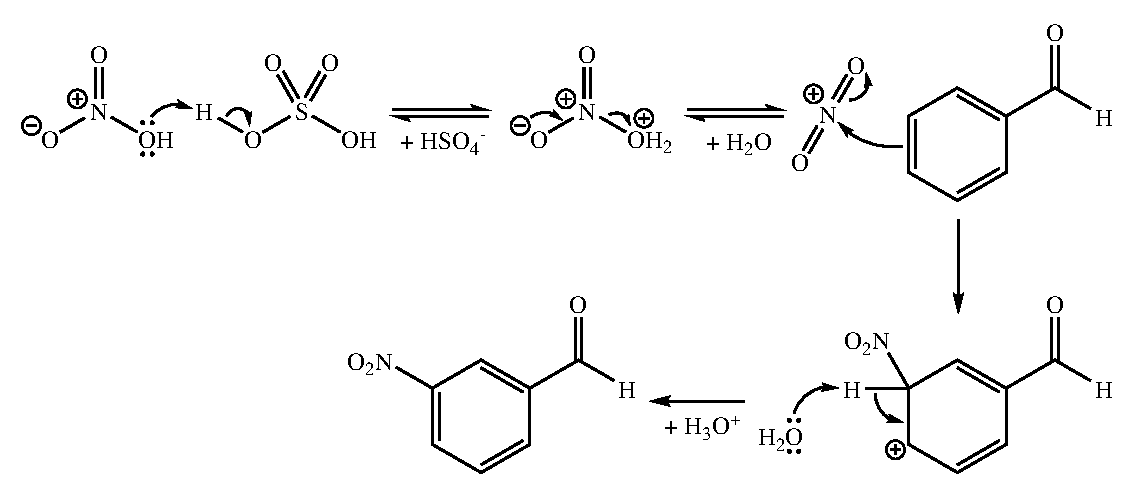
\includegraphics[scale=0.8]{mechanisms/nitration.eps}
    \caption{Mechanism of the nitration of benzaldehyde}
\end{figure}
\vspace{15mm}
\begin{figure}[h!]
    \centering
    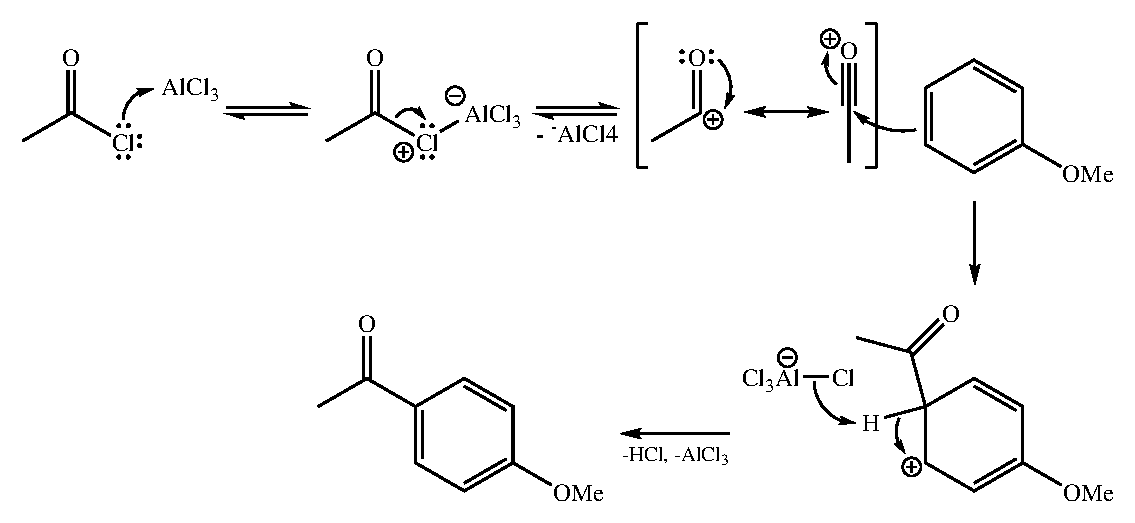
\includegraphics[scale=0.8]{mechanisms/acetylation.eps}
    \caption{Mechanism of the acetylation of acetophenone}
\end{figure}
\begin{figure}[H]
    \centering
    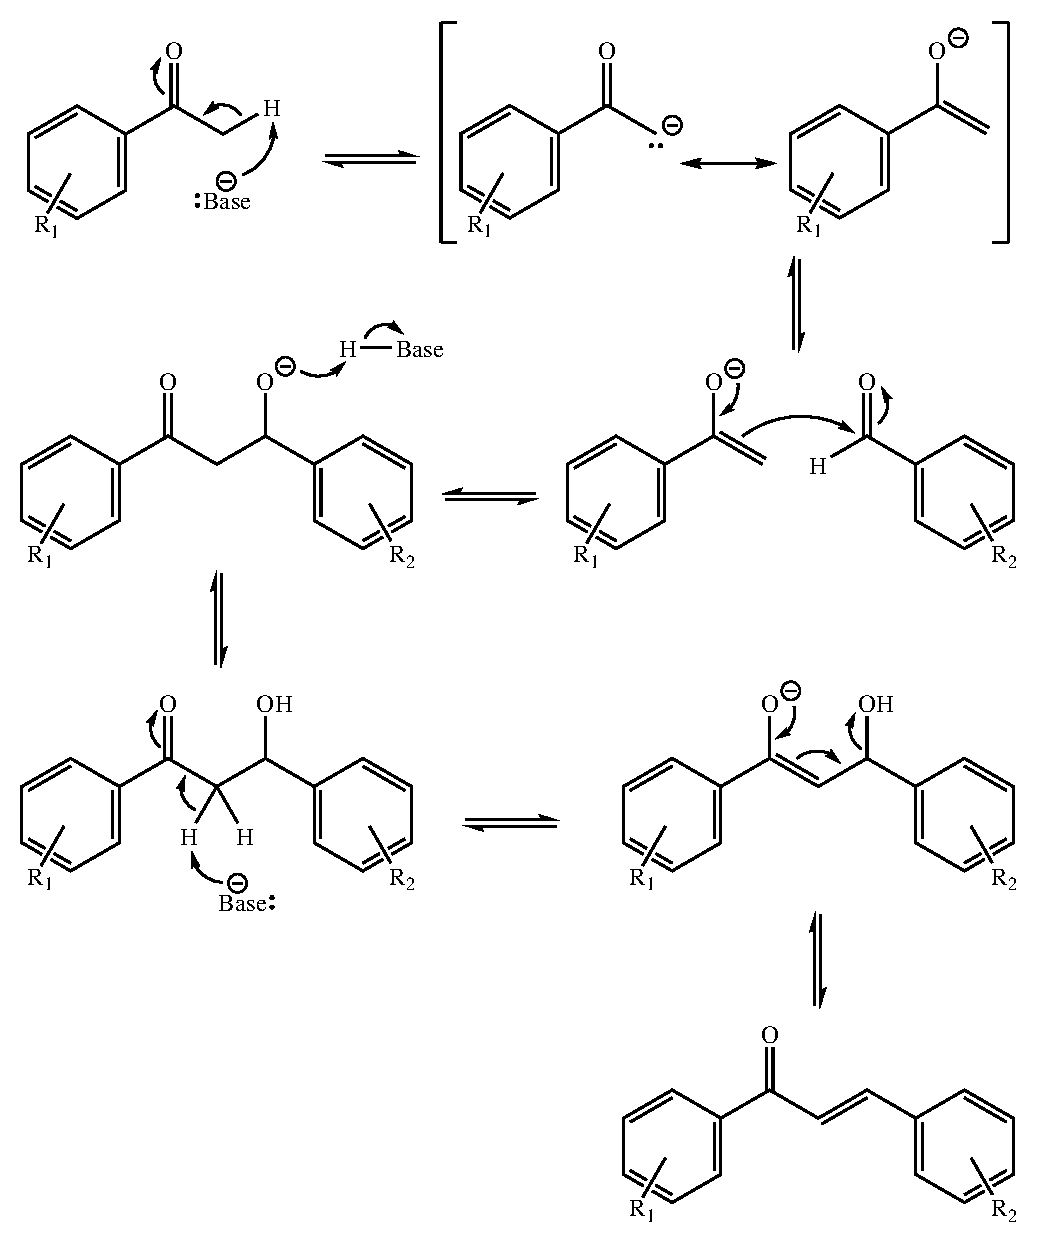
\includegraphics[scale=0.8]{mechanisms/chalcone.eps}
    \caption{Mechanism of the formation of chalcone}
\end{figure}
\end{document}